\documentclass[minf,twoside,singlespacing,parskip,frontabs,notimes,12pt]{infthesis} %

\usepackage{url}
\usepackage{subfig}
\usepackage{wrapfig}

\usepackage[xetex]{graphicx}

\usepackage{amsmath}
\newcommand{\BigO}[1]{\ensuremath{\operatorname{O}\bigl(#1\bigr)}}

\begin{document}
\title{Modelling search volumes as a dynamic system responding to external events}

\author{Stefan Sabev}

\course{Master of Informatics}
\project{{\bf MInf Project (Part 2) Report}}

\date{\today}

\abstract{
It is well known that certain events - football games, festivals, etc - spark people's interest to fly to different destinations. News events or sports events can quite easily make people search for a specific destination - for example the Champions League Quarter final draw increased the number of flight searches from Glasgow to Spain by a factor of 6.\\
The goal of this project is to prove that by taking social media into account, one can build a better model to predict flight search volumes.
For this project we have collected vast amounts of Twitter data. With this dataset and the flight search dataset provided by Skyscanner it was possible to build a model that predicts flight search demand based on what is happening on Twitter. This is a novel approach to predicting flight search volumes utilising the vastness of Social Media data available. 
The potential applications of this are generic prediction of flight search volumes, predicting new events for better marketing and also anomaly detection in traffic caused by events.
}

\maketitle

\section*{Acknowledgements}

This section will be kept brief. First of all, I would like to thank Charles Sutton for agreeing to supervise me on this project. Without his guidance, understanding and patience this would not have been possible.\\

I'd also like to thank Victor Lavrenko. He was my second marker and I received a lot of very valuable feedback from him and Charles that changed where this project was headed.\\

And last, but not least. Thank you Ewan Nicolson for guiding me towards this topic and sparkling my interest in the world of data.

\tableofcontents

\pagenumbering{arabic}

\chapter{Introduction and Background}

\begin{quotation}
"Prediction is very difficult, especially about the future.", \\
\textbf{Niels Bohr}
\end{quotation}

\section{Introduction}

We live in age of the "Big Data". 90\% of all the data we have ever generated on the internet has come into existence in the last 18 months to 2 years. 
The latest figures show there is about 2.5 exabytes of data generated every day in 2012\footnote{http://www.bbc.co.uk/news/business-26383058}. 
Undoubtedly with the advent of mobile services such as Snapchat, Wechat and many others, that amount has probably increased quite a lot. 
Most of this data of course is unstructured, comes in all shapes and sizes - pictures, videos and text. 
It ranges from the 350 million photos people are uploading to Facebook every day\cite{InternetOrgWhitepaper} to the 700 millions of photos disappearing from people's phones sent from snapchat\cite{snapchat}. 
Since all of it is human generated, there are now people in marketing and in data science who are starging to think of different ways to utilise the data. 

Therefore it should not come as a surprise that  companies living in this age of data are investing a big amount of money into analytics solutions that allow them to accurately predict their Key Performance Indicators (KPIs) - revenue, number of customers, profit, average purchase, etc. 
For companies living in the internet economy and the increasingly bigger sharing economy age it is of vital importance to be able to know on a daily basis how many customers you are expecting on the website tomorrow and a ballpark estimate of the average revenue per customer. 
The most important implication of those forecasts are budgets, but it could also be important for the company's operations. If there are people trying to access your website than what you usually have and the capacity is not there to meet the demand it will result in a crash that in turn will mean that you have foregone revenue. 
Perhaps one of the biggest high-visibility failures like this are the Obamacare website\cite{obcare} which went down, because of the high volumes of people trying to access it simultaneously to register  and the Black Friday crash of Best Buy\cite{bestbuy}. 
We are not arguing that the crashes would have been solely prevented by social media, because in the case of ObamaCare that was an one-off event. However both attest that being prepared is better than the consequences of being caught off guard. 

Precisely because of the unknown unknowns it is vitally important to make sure that the prediction mechanisms used in a company and the variables in them are going to reflect the environment accurately. 
If one solely relies on historical data without a holistic view of other variables, one would be able to create forecasts which do a very good job, but undoubtedly there will be a few cases where things go wrong. 
When you talk about the holistic view however, there is an another debate brewing - what exactly to use to provide that view. Of course one can use news sources - RSS aggregators, news website, TV or any other traditions media which can be used to inform the person making the prediction of anything that could affect it. 
That approach is resource-intensive and prone to errors, because those events might not impact the way it is been thought. But there is an alternative - Social media. 

With hundreds of millions - and in the case of Facebook, billions - of users, social networks have become an inherent part of our daily lives. Something that was not imaginable 10 years ago is now indispensable. 
We ``tweet", we ``snapchat", we chat to people on ``whatsapp", post our latest holidays photos to Facebook, declare where we are going to eat on Fourqsquare and soon as we go in we Instagram our food. 
In a matter of a decade people have become perfectly fine with externalising their lives to an incredible degree and posting every minute detail online and making it available to friends and in some case - the whole world. 
It is not to say that absolutely every one does. 
After all, 80\% of the world is not on Facebook\cite{FBstats}, however the 1.31 billion monthly active users are all sharing some data about themselves. 
We are increasingly transferring more and more of our personalities online.
 With this amount of data on one's behaviour, life patterns and activities, companies can build a very good understanding of every individual and potential customer.


This project was born after a discussion into the benefits of Social media and how it can be used in a business context. 
The most popular uses of Social media at the moment are Sentiment analysis and targeted advertising. 
Sentiment analysis is basically putting the mentions of your brand/company into two big buckets - positive or negative about a brand, topic or something else you want to measure against.
Targeted advertising on the other hand is just matching the right people with the advertisements that are supposedly the most relevant for them. 
Skyscanner already uses both as a company so we tried to come up something novel. 
That novel idea was to use some external data taken from a social network that we can use an external factor in our predictions. 
Hence the searches become the dynamic system that reacts to the external factor when the factor can play a big part. 

The social network which we are using for this research is called Twitter. 
It has a base of about 288 active million monthly users.
Those 288 millions users produce over 500 million tweets every single day\footnote{https://about.twitter.com/company}. 
It was viewed as a replacement of text messages - hence why the limitation is 140 characters - but it has grown to be one of the most prominent sources of information and news on the web. 
Since old media such as TV, newspapers, etc require some form of approval or preparation Twitter often beats tradition news sources by a some margin. 
For instance when the Los Angeles earthquake happened in 2008\cite{TwitterNewsWire} Twitter reacted seconds afterwards, while traditional media took 4 minutes. 
The fact that they have public streams open to developers and researches makes it the best candidate social network to use. 


There were several options that will allow us to add that externality - news sources (RSS, news websites) and social media. 
Of course not all social media websites have got public websites and the ones that do impose quite a lot of restrictions. 
After some initial evaluation it was decided to go with Twitter, since the Public Streaming API, which is a 1\% stream of the data they offer will allow us to easily access the data programmatically and the data volumes mean that the sample size would be good. 


Since this is the second part of the project, we have already done a sizeable amount of work in year 1. 
In the first part of the project we build all the underlying code that allows us to easily process the Twitter Stream, save it on disc and then extract the data we need from it. 
We will go into more detail on what work was done in Chapter 2 - Summary of Phase 1. 


\section{Discussion of related work}

Contrary to many other areas of computer science, there is not an established body of literature that is particularly concerned with prediction using social media and unstructured data of this particular format in the airline world or for predicting flight demand in any form. 
However that is not to say that there are no previous attempts to use the wealth of Twitter data and put that to use in some context. 

Petrovic, Osborne and Lavrenko\cite{Miles2} have tried predicting whether a Twitter message will be deleted. 
They trained an Support Vector Machine and used the Passive-Aggressive Algorithm to train a linear classifier. 
The authors had 72 million tweets which they acquired over the course of a month and from that they extracted about 42 million features. That proved to be quite a big number for the SVMs they wanted to use for classification so they had to resort to the Passive Aggressive algorithm. The results they reported were good, since it showed that Twitter data can be used for more than just trending hashtags and finding out where people tweet from. 
An exemplary research into Twitter is Sasa Petrovic's PhD thesis - ``Real-time event detection in massive stream"\cite{Petrovic2012}. 
In this work the author has done extensive research into the role of Twitter as a news wire and whether it can beat traditional news outlets. 
In majority of the cases the traditional media still wins by a big margin and where Twitter is first it turns out it's not first by much. 
 Therefore Twitter can indeed be used to predict demand or at least events. 
 In this work we're not concerned with predicting it as soon as possible, but rather seeing how it influences demands for flights on certain routes.

The quote at the beginning of the this chapter by the famous Niels Bohr is a general summarisation of the difficulty of prediction. The process is hard enough on its own, but when you add a noisy channel like Twitter where distinguishing the signal from the noise is hard and unfortunately you are only making things worse. Some of the most interesting uses of Twitter in research are Bollen and Mao trying to predict the stock markets\cite{twitstock}, Sinha et al predicting the outcomes of NFL games\cite{twitnfl}, looking into predicting the poll outcomes\cite{twitpoll} and looking into the overall health of the nation in Paul and Dredze\cite{twitflu}.


The first paper that we will review is Bollen and Mao\cite{twitstock}. 
The finance world has never lacked resources and it's know for attracting bright minds from many disciplines to try to extract more value out of different mediums in order to aid their knowledge of the market which can essentially be boiled down to whether a stock will go up or down. 
There has been a lot of work done on whether news can predict where the market is headed, all with varying degrees of success. 
In this particular paper the authors are looking at the Dow Jones Industrial Average \cite{dija} (DJIA or DOW as the investors affectionately refer to it) and whether Twitter can aid in predicting its daily fluctuations. 
They are doing that based on investor mood since that is considered to be  one of the best predictors - if investors are happy or have a positive outlook on things, the stock markets rally and vice versa. 
In order to do that, they used Opinion Finder (OF)\cite{opfind}, which measures opinion the same way one would perform sentiment analysis - bucketing into either positive or negative. 
That was found to be rather insufficient, since human moods are much more complex than a simple binary model. 
They developed their own system called GPOMS that will help them capture that complexity. 
It splits the investors' sentiment into 6 distinct emotions rather than just two.
In the paper they prove that the GPOMS values are much more predictive than the binary OF values. 
As we all know, correlation does not imply causation and in order to verify that they carry out a Granger causality analysis\cite{granger}, which rests on the assumption that if X causes Y then, as one would expect, changes in X will systematically occur before any changes in Y. 
An important note is that in most similar projects and indeed in this one, we cannot prove actual causation - 'happy' or 'angry' causes the stock market to go either way - but rather we are simply trying to verify whether the data we have is predictive of the value we are trying to forecast. In this case it is checking whether the public mood time series for the different moods can explain the fluctuations in the DJIA. 
After checking all different moods, the results showed that Calm and Anxious are the moods that have the highest predictive values. 
For the actual prediction they used a Self-Organising Fuzzy Neural Network (SOFNN) \cite{sofnn}, which is a five-layer hybrid neural network, which with the ability to organise its neurones during the learning process. 
As a result the values Calm and Anxious can predict the market movement with 90\% accuracy. 


There is definitely a good argument to make that using Twitter for predicting the stock market. 
Some companies such Bloomberg are now packaging that data and transforming into a product that they sell to financial institutions.\footnote{https://gigaom.com/2015/02/03/as-social-media-gets-quantified-more-people-use-twitter-to-trade/}. 
In the above mentioned paper the authors make a strong case that capturing public sentiment can be indeed used to show where things are headed. 
As far as their methods are concerned, we did examine neural networks, however the overheard of training them, tuning the parameters and the fact that we are dealing with time series data lead us to think that they are perhaps not the best suited tool for this particular type of prediction. 

In Bollen and Mao\cite{twitstock} there was a clear relationship between mood and the stock market, however one can argue that there are other factors that influence the direction of stocks. 
Twitter is an expression of public opinion on a variety of topics, so it is not surprising that it can be used to predict public opinion on a vast range of topics like in O'Connor et al\cite{twitpoll}. 
In the paper the authors make a strong argument that using Twitter one can predict public sentiment just as well as the poll, but it does not suffer from the poll's problems - being very expensive and time inefficient. 
Since polls are a lagging indicators Twitter can completely take over in that space accuracy permitting this.
The authors used the garden hose Streaming API of Twitter from the beginning of 2008 until the end of 2009. 
In the time period of scraping the number of daily tweets has increased by a factor of 50, due to the fact that Twitter has had an exponential user growth at the time.

In order to filter out the data, the authors looked for keywords:
\begin{itemize}	
\item For consumer confidence - \textit{economy}, \textit{job} and \textit{jobs};
\item For presidential approval - \textit{obama};
\item For elections - \textit{obama} and \textit{mccain}.
\end{itemize}

Afterwards by mining the tweets they obtain the time series for Twitter in a very similar fashion to what we have done in this work. 
Since Twitter data can have a lot of spikes, something that we have experienced throughout this research as well, the authors remove those outliers by using a moving average. 
They call it "Moving average aggregate sentiment", which smoothens the volatile daily variations, but at the same time does not remove the fine grained changes in public sentiment that the polls try to capture. 
They use different values - 1, 7, 30, which is basically no smoothing, smoothing back a week and smoothing back a month. 
With the different values they achieve different levels of correlation with the public opinion polls all sitting at about 70\%. 
We have also explored smoothing out our data and it was shown that by weekly smoothing we achieve maximum correlation without removing the intrinsic seasonality of the data.

They also use the time series data for prediction as well. 
The authors have picked the Linear Least Squares model with a lag hyper parameters. 
The model is trained on the smoothed data and then they just measure the correlation with the actual poll numbers to see whether the forecast is good enough to supplement or even supplant the polls. 
The authors comments are quite interesting - in 2008 the \textit{r} (Pearson correlation coefficient) for the election polls was -8\%, which is insignificant. 
However, they note that in 2009 Twitter becomes a much better prediction achieving \textit{r} from 44\% to 57\% with different lag coefficients. 
That reflects on the fact that perhaps in 2008 as a relatively new service, Twitter was not used by many, but later on as adoption increases, the way people use the service changes and as more people use it will become a better indicator for consumer confidence and also election polls. 

Another area where researchers could benefit from Twitter is something that has already been done before by Google - predicting flu outbreaks and public health in general. 
Google uses searches from their search engine, while Paul and Dredze\cite{twitflu} use Twitter to paint a picture of how public health looks like the United States. 
A big proportion of Twitter users come from the US and the geo-tagging option allows you to see where the person is tweeting from, therefore you can see what is happening on a very granular level. 
The authors make an argument that Twitter, unlike Google, can be used for much more than influenza tracking. 
They hypothesise that with the help of that social data, one can analyse how diseases spread, how fast they are spreading geographically and also what demographics are influenced by it.


In order to get started with the models they use something which they call Ailment Topic Aspect Model (ATAM), which is an extension of a Latent Dirichlet Allocation\cite{lda}. 
After they trained the models with the different topics they run a simple correlation test on the Center for Disease Control and Prevention (CDC) FluView which tracks flu across the states. 
The results they posted are very good - correlation coefficient of 0.958. 
To put that in perspective, other studies post results around 0.96 and 0.97, however the major difference is that they train their models on the government data and only look for flu-related terms on Twitter, while in this study they use a generic model that learns about different disease one of which is Twitter. 
Thanks to the geotagging features the authors go on to see how diseases spread throughout the year and what are the most common symptoms by month and by state. 
There is definitely a strong case here that shows the versatility and the breadth of the data they have collected. 

In all of the above mentioned papers the authors were using the treasure trove of data to predict something that can be directly influenced by the people on Twitter - be it public polls, be it public health or to some degree the market. In Sinha et al\cite{twitnfl} there is a radical departure from that where the authors are trying to predict the outcome of an NFL game based on the different tweets about the game. This showcases the limitations of the dataset - even with their most sophisticated methods and cherrypicked features they still managed to achieve prediction accuracy of 50\% which is no better than a coin toss, however that should come as no surprise. After all in all previous studies the people who use Twitter are part of the mass that influences the measures the authors were trying to predict - be it directly or indirectly. However in this case we are using the data to predict something that is not directly influenced by the people using it - unless of course we select a team of highly-trained pundits who do that for a living, but even then some studies show that the accuracy is still going to be comparable as when we base our decision on a simple coin toss.  

All of the papers mentioned above are showcasing the versatility and the plethora of ways that Twitter can be used to predict various different things - ranging from public health going all the way to football games. 
A lot of people post a lot of their daily schedules and lives on Twitter so in this work we will try to see how Twitter can be used to better search volumes forecasts. 


The most researched thing in the airline sector so far has been finding the optimal time to book an airline flight\cite{Hamletkdd03,ijcai}. 
At Skyscanner there has been a lot of research into this with a lot of tools helping you to find the best time to book your flights \footnote{http://www.skyscanner.net/bttb/best-time-to-book-uk/}, with the obvious caveat that if everyone goes to book in that optimal for now time in the very near future it will not be optimal at all. 
Other areas of aviation research include: competitiveness, the influence of hub airports and how they affect competition, airline alliances and whether they are good for the customer and others. 


The considerations of aviation research however are tangential to the work in this project. 
They are more concerned with the implications of what we currently have, while we are more interested in making predictions for the future. 
Here we are exploring whether the data obtained from Twitter can improve the forecasting methods used at Skyscanner and whether we can create a change point algorithm that uses both the flight searches data and the Twitter data. 

\newpage
\section{Summary of contributions}

\begin{itemize}
\item \textbf{I developed a scalable system for storing, analysing, exploring and visualising the data.}
\item \textbf{I suggested, explored and implemented a novel way of predicting flight search volumes with taking exogenous factors into account.}
\item \textbf{As a result of my models I have managed to improve overall prediction of flight search volumes by 5\%. As a side effect we also saw the effects of events such as the Winter olympics and the riots in Ukraine.} 
\item \textbf{Developed a new offline and online algorithm that can be used with any model to see whether a change point occurs in a stream of time series data. The online algorithm helped to improve forecasts by segmenting the time series into regions that we could fit models on.} 
\item \textbf{Compared and benchmarked a variety of models against each other and determined which was the best for forecasting flight search volumes. The best performing setups were the ARIMA change point detection + ARIMA and the Bayesian change point detection with ARIMA.}
\item \textbf{Explored how Twitter can be used to improve forecasting and how to incorporate social data in forecasting}.
\end{itemize}



\chapter{Summary of Phase 1}

There was a clear purpose, which we had in mind at the beginning of the first phase of this work - to change the methodology that Skyscanner uses to forecast flights search volumes. We can say that this has been achieved. Some of the work has been used directly, while the parts that have not been used sparked discussions. At the beginning of the project there was one method used - a simple classifier looking only into historical data without any assumptions. Now Skyscanner employs a lot of different methods which means that the quality of the forecasts does not depend solely on 1 number. 

The plan we had set was:
\begin{enumerate}
\item Create an extensible and modular set of tools that will allow us to do all of the needed tasks:
\item Collect data from the Twitter API and the Skyscanner database. 
\item Process the data and convert it to time series.
\item Explore the correlation between the time series from the two datasets
\item Cleanse all the problematic elements by either backfilling where possible or by removing them.
\item Extract the features for the multi feature models.
\item Then start building the models, collect data and analyse it. 
\end{enumerate}


We did stick to this original plan. The tools we created \cite{code} are very effective at gathering, extracting, processing and building the automated models. Unfortunately, by the time we finished building all of them and tidying up the code that was training and outputting the models there was not much time for statistical analysis. That in turn meant that the first phase did not have the right amount of in-depth reflection and justification of the design features.

\section{Collection}

Machine Learning requires data to learn from. As such, first and foremost one has to collect the data that one needs and the data that one can. For this project the time series of Skyscanner flight searches and the Twitter data were used.

Since I am a Skyscanner employee working in Analytics, the flight searches were quite easy to obtain. In order to keep the data on the number of searches confidential we have normalised them as having 1 as the maximum value and everything else is a proportion of that. 

The data obtained from all the SQL querying was the searches time series for 2403 destinations. Those destinations are all the cities with an airports and countries that you can fly to. The time series are stored in a Comma Separated Values (CSV) files, named after the destination which contains the data aggregated on a daily basis as shown in Table \ref{ssearches}. In order to remove any concern with confidentially we have anonymised the data when plotted or removed the axis labels altogether when plotting the actual values.

On the other hand Twitter's Public Streaming API was not something that we have previously worked with. Our initial estimation was that we would be receiving approximately 1.5 gigabytes of data a day based on daily tweet numbers and multiplying it by our rough estimate for the maximum size of a tweet. After running the collector script for a day that number turned out to be very close to 6.5 gigabytes. Since not all of it was data that we were particularly interested in - pictures, videos, interactive content - we decided that it was worth to have a read at the documentation and see what exactly is included in a tweet.  After careful consideration we picked the attributes, which we needed now and the ones that could be beneficial in the future. By selecting those particular we managed to reduce the daily volume of data from 6.5GB to 3.5GB a day, which is a reduction by factor of 2. 


\begin{table}[h]
\begin{center}
\begin{tabular}{ l | r  | r }
\textbf{Date} & \textbf{Searches} & \textbf{Tweets} \\ 
\hline
2013-09-25 &  X  & A \\
2013-09-26 &  Y  & B \\
2013-09-27 &  Z & C \\
\end{tabular}
\end{center}
\caption{Time series format used in the dissertation}
\label{ssearches}
\end{table}

Since Twitter has experienced a phenomenal growth the cut down data we collect daily has grown itself from 3.5 GB/day to 15GB/day. The data accumulated at the time of writing is 1.8 TB of textual data that contains around 2 billion tweets. As mentioned at the beginning of the chapter, we have collected data since the 24th of September 2013 until December 2014 with an interruption during the summer months. Due to some network outages, buffer overflows, etc, there are some holes in the data, so it is not as consistent as we would like it to be, but we have dealt with that by cleansing the data prior to training and evaluating my models. 


All in all, data collection was probably the easiest of all the different sub-tasks, but at the same time it was the most important one, because everything else in this project depends so much on the data gathered. We believe our solution was simple enough, because for 6.5 months, we have got less than 10 days with gaps for the days that it was running . That is less than 5\% of the overall collection time. In those gaps, the failure of the collections was caused by human error or network interruption or a failure, because of the Streaming API. 


\section{Processing}


With the foundations of the project in place and the data flowing in into text files comes the next part of the project - processing and extracting all the relevant parts from the messy, unstructured stream. 

There were 3 options for the data processing and storage:
\begin{itemize}
\item Storing it in a relational or noSQL database and processing it that way. 
\item Using a Hadoop cluster for the storage and processing. 
\item Storing in flat-text files and processing it with custom scripts.
\end{itemize}

After evaluating the options, a database was immediately ruled out. Relational databases have very poor handling of text, while noSQL ones tend to be very bad in terms of programmatic support. Hadoop seemed very fit for the job, but due to the fact that we had no working experience of it, we made the decision not to use it. The third and last option seemed to be the most feasible one. Therefore, we built a toolset of various Python scripts that did all of the various parts needed to run an end-to-end experiment - collection, processing and training the models and evaluating them. 


Finding out what keywords to use was the next logical step. In Twitter there are two ways to approach the problem:
\begin{enumerate}
\item Use only the hashtags  - words preceded by a \#.
\item Use all the words in the tweet.
\end{enumerate}

The simplest way to go about solving this problem was to extract the hashtags, since that requires no text processing. Twitter already ships the hashtags as a separate data structure within the tweet, so processing those requires just taking them and storing them in a dictionary with the counts. However, since we are concerned with place names it turned out that the volumes of place names that have been hash tagged was not sufficient.

Therefore we had to go for the second option - process the whole tweet and extract the relevant place names and time series from it. That of course meant additional processing time, since for every word in the tweet we had to check whether that word is a place name or not and then to see whether the tweet contains any travel words. After coding up the solution, we discovered that the volumes of the simple word counts were sufficient and were not prone to any explosive fluctuations as with the hashtags.

 The processing of the data itself was relatively simple - we have 2 dictionaries that hold the place names and the travel words. Each words is checked against those dictionaries, since dictionary lookup is O(1) therefore the complexity of the whole lookup for a tweet is O(n) where n is the length of a tweet. For every day and words we hold a separate counter in the dictionary that gets 1 added every time we see an occurrence. After a simple transformation we output what can be seen in Table \ref{ssearches} to obtain the final time series data. 
 
 For the later models we used all the words that co-occur with a place name as additional features, but that requires no significant changes to the data processing tools. 


\section{Automated models}

The baseline model that we set out to beat in the first phase of the project was a simple exponentially weighted moving average that follows the following formula:
\begin{equation}
\tau=0.675*(\tau-7) + 0.225*(\tau-14) + 0.075*(\tau-14) + 0.025*(\tau-21)
\end{equation}
where $\tau$ is the value for the day we want to predict, $\tau-7$ is the value for this day of the week from last week and so on.

This basic model performs quite well and has been used for a year or so, because it significantly outperformed the simple Excel spreadsheet that was used before. 

In total, there were about 1600 models trained that were models of the search volumes as a function of twitter and the previous dates for every city or country that one can fly to. All of those models were LASSO because it both picks the optimal weights but it can also make a prediction for the values as well. This proved that LASSO was the best choice at the time to create this large system that extracts, processes, trains the models and forecasts the future data. 

Throughout the training process we used a standard 80/20 split, where we used 80\% of the data to train the models and the other 20\% of the data to assess the performance of the models. 

\section{Models with additional features}

As mentioned above in the processing section of the report we also extracted the full set of words co-occuring with place names and used those as well. That was interesting from a different point of view, because when we trained the models we saw which words have the highest weights, meaning that the words with the highest weights had the biggest predictive power. In Table \ref{tab:sochi-table} you can a few of the features that LASSO picked for the Sochi model. The influence of the Olympics can be clearly seen. 


\begin{table}[]
\begin{center}
\begin{tabular}{l | r}
Feature & Weight\\
\hline
team & 16.08\\
\#olympics2014 & 2.40\\
Count & 1.34\\
olympic & 1.30\\
canada & 0.72\\
hotel & -1.07\\
\#seeyouinsochi & -1.22\\
jump & -1.49\\
\#olympics & -2.24\\
dog & -2.56\\
sochi & -2.52\\
\end{tabular}
\end{center}
\caption{Handpicked features for Sochi. The total number of features is 44 and they are the ones picked by the model. } 
\label{tab:sochi-table}
\end{table}

The models with the extended feature sets did not perform as well as we expected reducing in decreased performance and increases Root Mean Squared Error (RMSE) across more than 90\% of destinations.


\section{Conclusion and results}


The first phase of the project was a hybrid between systems and a scientific project. That resulted in perhaps a bit of a dilution in the effort, since we were trying to both create the extensible toolset and work on the modelling side as well. 

In Table \ref{big-table} we present the results of the top 10 destinations sorted by RMSE. As we can see for the majority of destinations there was a minor improvement and overall we have achieved a reduction of the RMSE by 5\% across all destinations, which then in turn allows for more more accurate revenue forecasting as well. 

\begin{table}[h!]
\begin{center}
\begin{tabular}{ l | r | r | r }
Place & RMSE Skyscanner & RMSE Twitter  & Improv\\
\hline
Spain & 85,844 & 78,424  & 8.64\%\\
US & 78,480 & 73,581   & 6.24\%\\
UK & 68,706 & 65,696  & 4.38\%\\
Italy & 54,804 & 53,020  & 3.26\% \\
London & 40,129 & 39,222& 2.26\% \\
Russia & 38,712  & 36,033 & 6.92\%\\
Germany & 36,113 & 35,137 & 2.70\% \\
France & 34,020 & 32,816  & 3.54\%\\
Thailand & 29,997 & 30,374 & -1.26\%\\
Turkey & 29,616 & 28,316  & 4.39\%\\
\end{tabular}
\end{center}
\caption{Comparison of the RMSE of the Twitter model and the Skyscanner forecast method for the top 10 places sorted by descending RMSE. }
\label{big-table}
\end{table}

\chapter{Models}

In this section we will give a brief introduction to the different models that we have used for this project. I have provided an overview of the incumbent, which we are trying to improve on and also the contender and why it is a better suited candidate for the job. 



\section{The baseline}

Even though that now this is no longer the case, at the start of this work, Skyscanner did not have a very sophisticated toolset for forecasting. They have now fully transitioned into automated forecasting with a suit of tools, that cuts the data several different ways, but at the time they had a spreadsheet and a simple model called Last 4 Fridays. Last 4 Fridays is a very simple version of an exponentially weighted moving average, where you are looking at the same at the same days of the week from the past 4 weeks and assigning different weights to each of the previous days of the week. The weights are exponentially distributed and the formula is defined in Equation 2.1.


It is a very primitive model in compassion to Holt-Winter, ARIMA or any other form of regression/forecasting models. However it is good enough for the following reasons:
\begin{enumerate}
\item There is no training overhead at all  - with ARIMA, Holt-Winters, Vector Autoregressive Models, one has to find the optimal parameters and those would be different for different destinations and if we want to predict overall search volumes. With the L4 there is still a certain tweak to the parameters, but the the first day has 3x the weight of the one after and so one. All of the weights sum up to 1.
\item Also much simpler to maintain. The other models might require tweaking every now and then, while this can run on auto-pilot and there will be no significant maintenance.
\item Because of the weighting scheme it captures seasonality - the most recent data point has a weight 3 times higher than the others, so  because of that it will be the biggest contributor to the final value; 
\item The fact that the RMSE was on par with the other more sophisticated models and it required no additional work. 
\end{enumerate}

Of course, there was an even simpler version considered - taking the data from the same days of the week from last week and multiplying that by a constant. That produces excellent results and did have the smallest overall RMSE, but in the quite likely event of an outlier the results are absolute rubbish and if there was a football match last week for instance with an increase of 1.5 times the number of searches you would usually have next week will look very similar to that without any justification. 

Therefore for the time being Last 4 Fridays was providing the optimal tradeoff of accuracy and work needed to produce the forecasts/to maintain. 

\section{LASSO}

The LASSO (Least Absolute Shrinkage and Selection Operator) is the model that was used in the last phase of the project. We need a model that will be good at selecting weights from the plethora of features, but also was good in the forecasting and easy to implement.  Another major problem of the first phase was that we hurriedly try to add the Twitter data without much correlation. For over 80\% of the destination the Pearson tested yielded a correlation coefficient of $<0.5$, which is a pretty low correlation as far as we concerned. That is precisely why we did not build any models that were solely using Twitter to forecast the flight search volumes. Instead they were helped  by it. The features we used for the models were ranging from the Fridays as they are present in the Last 4 Fridays baseline and a count of the number of times a place has been mentioned on Social media to the full set of words co-occurring with the place we are building the model for. 

As an experiment, we also had 2 different models - one where the weights for the Fridays are predetermined and one where they are picked by the LASSO model. Both ended up working quite well, but there was not a big difference in the results from both. 

The way that LASSO works is that it picks the optimal weights for every feature by minimising its objective function:
\begin{equation}c
\underset{w}{min}({\frac{1}{2n_{samples}}} \|X*w - y \|_2^2 + \alpha\|w\|_1)
\end{equation}

It is essentially a liner model with l1 regulariser. It solves the minimisation with the least-square penalty for $\alpha\|w\|_1$ where $\alpha$ is the regularisation parameter and and $\|w\|_1$ is the l1 norm of the parameter vector. In last year's case for the simpler models we did not experiment too much with $\alpha$ but for the models with thousands of features we observed that the more you increase $\alpha$ the more the junk weights are penalised hence it prefers sparse solutions with sparse coefficients. 

In general the model worked quite well and the improvement in forecast was 5\%. However we needed to combine that with some more detailed understanding and alerting of when events happen. 



\section{ARIMA}

Unlike last year where we just trained a lot of models using LASSO, this year we decided to take a more theoretical approach and try to understand a bit more before approaching it with random models. Out of the few candidates that we benchmarked the AutoRegressive Integrated Moving Average (ARIMA) was the best performing one, since it's is developed to take into account seasonality and exogenous factors. 

Due to the very seasonality of the data and its trends, ARIMA is perhaps the best model for this job. The model is generally referred to as ARIMA(p,d,q) since p, d and q correspond to the three parts of the model - the auto-regressive (p), the integrative (d) and the moving average (q).

The ARIMA formula is the following:

\begin{figure}[h!]
\begin{center}
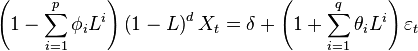
\includegraphics[width=0.7\textwidth]{ARIMA}
\end{center}
\caption{ARIMA formula. Given a time series of data $X_t$ where t is an integer index and the $X_t$ are real numbers. L is the lag operator, the $\alpha_i$ are the parameters of the autoregressive part of the model, the $\theta_i$ are the parameters of the moving average part and the $\varepsilon_t$ are error terms. The error terms $\varepsilon_t$ are assumed to be independent, identically distributed variables sampled from a normal distribution with zero mean.
}
\label{arima}
\end{figure}

That means that there are three parameters that need to be found. In order to find those parameters we have 2 different options:
\begin{enumerate}
\item Do it from inferring optimal parameters from the autocorrelation and partial autocorrelation plots.
\item Use the available auto.fit function.
\end{enumerate}

\subsection{Autocorrelations}

In the world of statistics, there are a lot of different best practices that can seem perhaps a bit unintuitive to an outside. Picking the ARIMA parameters is one of those. What one does is plot the autocorrelations and the partial autocorrelations for the series - be it uni- or multivariate - and then based on the confidence bands pick the autoregressive order that is deemed to be the best for the job. Of course it is always helpful to plot those, but perhaps picking the parameters solely on that is something that should be left to more seasoned practitioners, who have the experience and intuition to pick them easily by just looking at those 2 plots. 


The autocorrelation plot for Sochi ca be found in Figure \ref{autocor}  and the partial autocorrelation in Figure \ref{megacor}. In our case we can see that the Searches autocorrelation are statistically significant until the a lag of 20. Searches and count are correlated until a lag of 10. That means a autoregressive model is a very good candidate for the job. 


\begin{figure}[]
\begin{center}
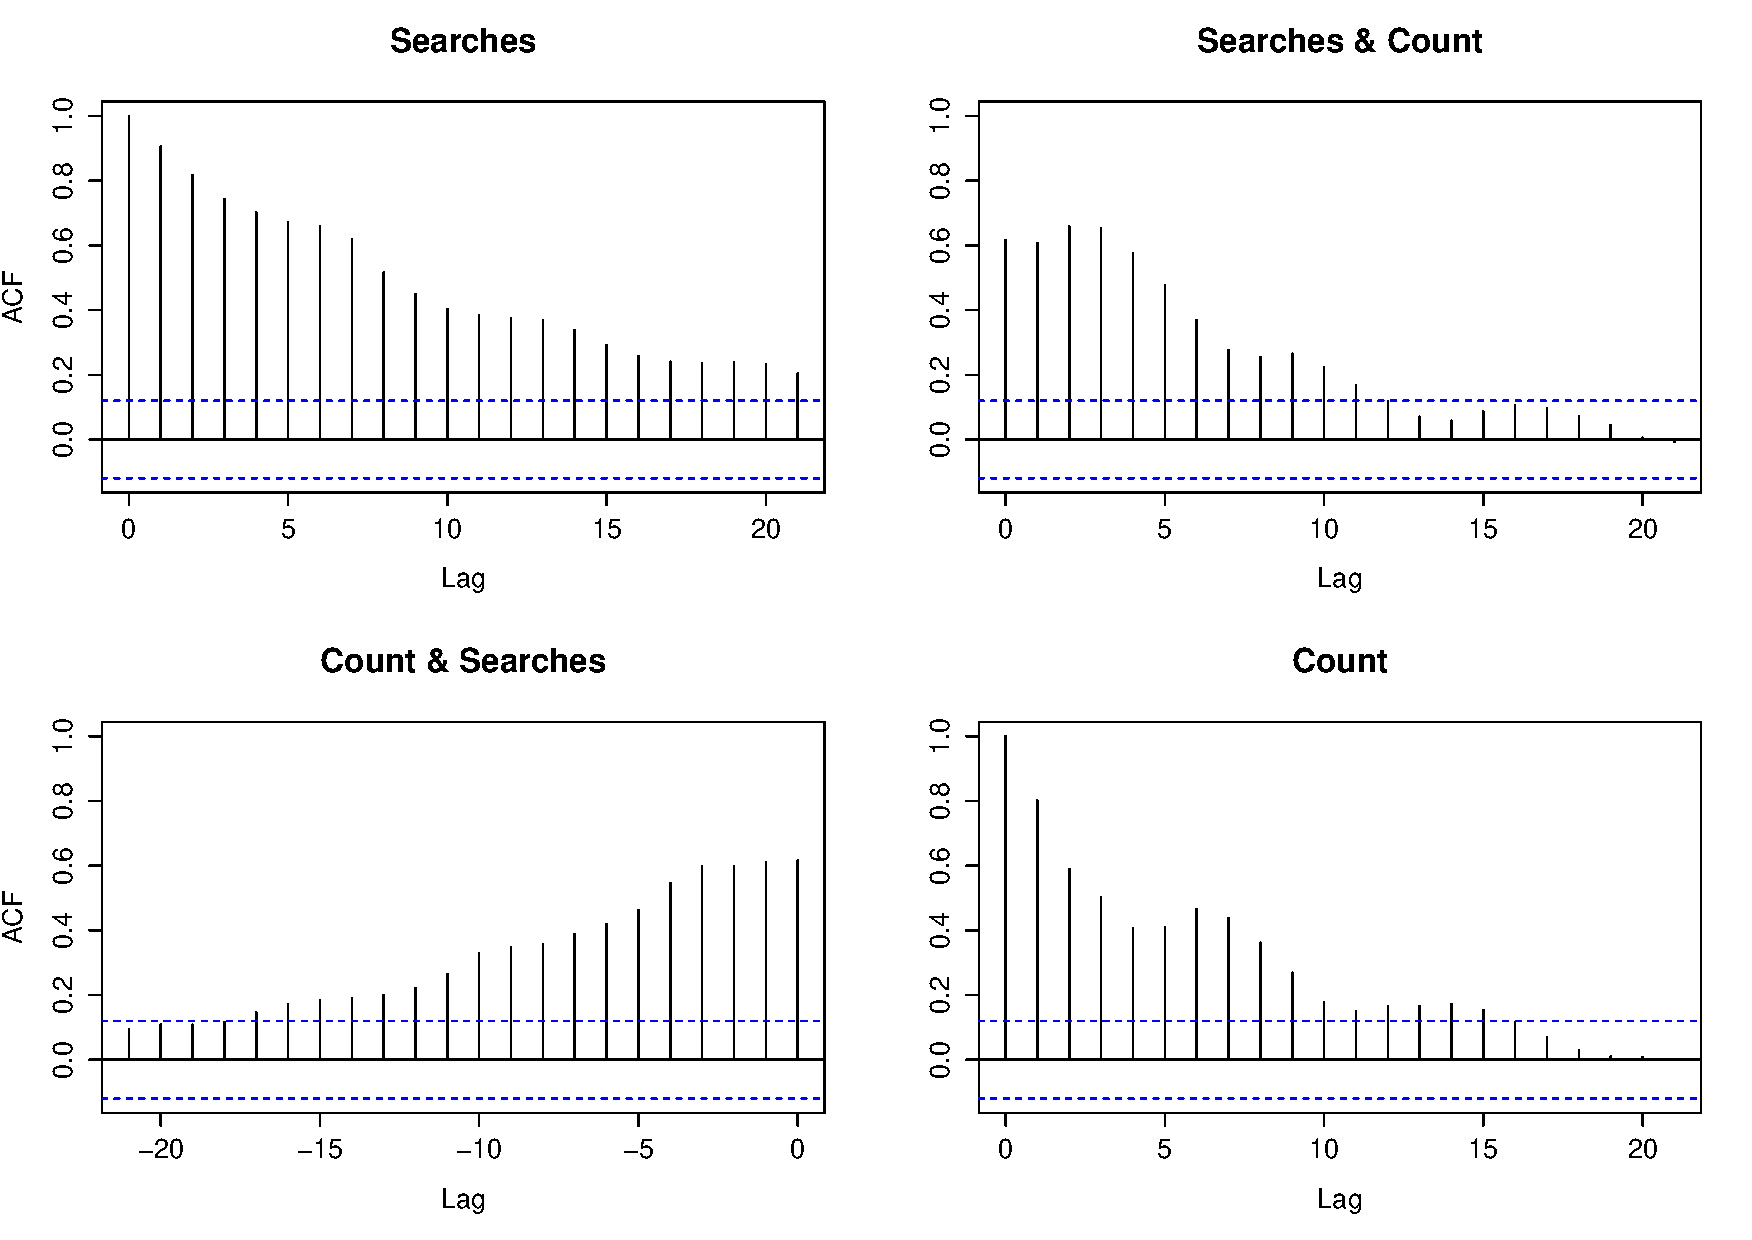
\includegraphics[width=\textwidth]{autocorrelation}
\end{center}
\caption{Autocorrelations for the data set. The blue dotted line is the 95\% confidence level, anything above is statistically significant.}
\label{autocor}
\end{figure}

\begin{figure}[]
\begin{center}
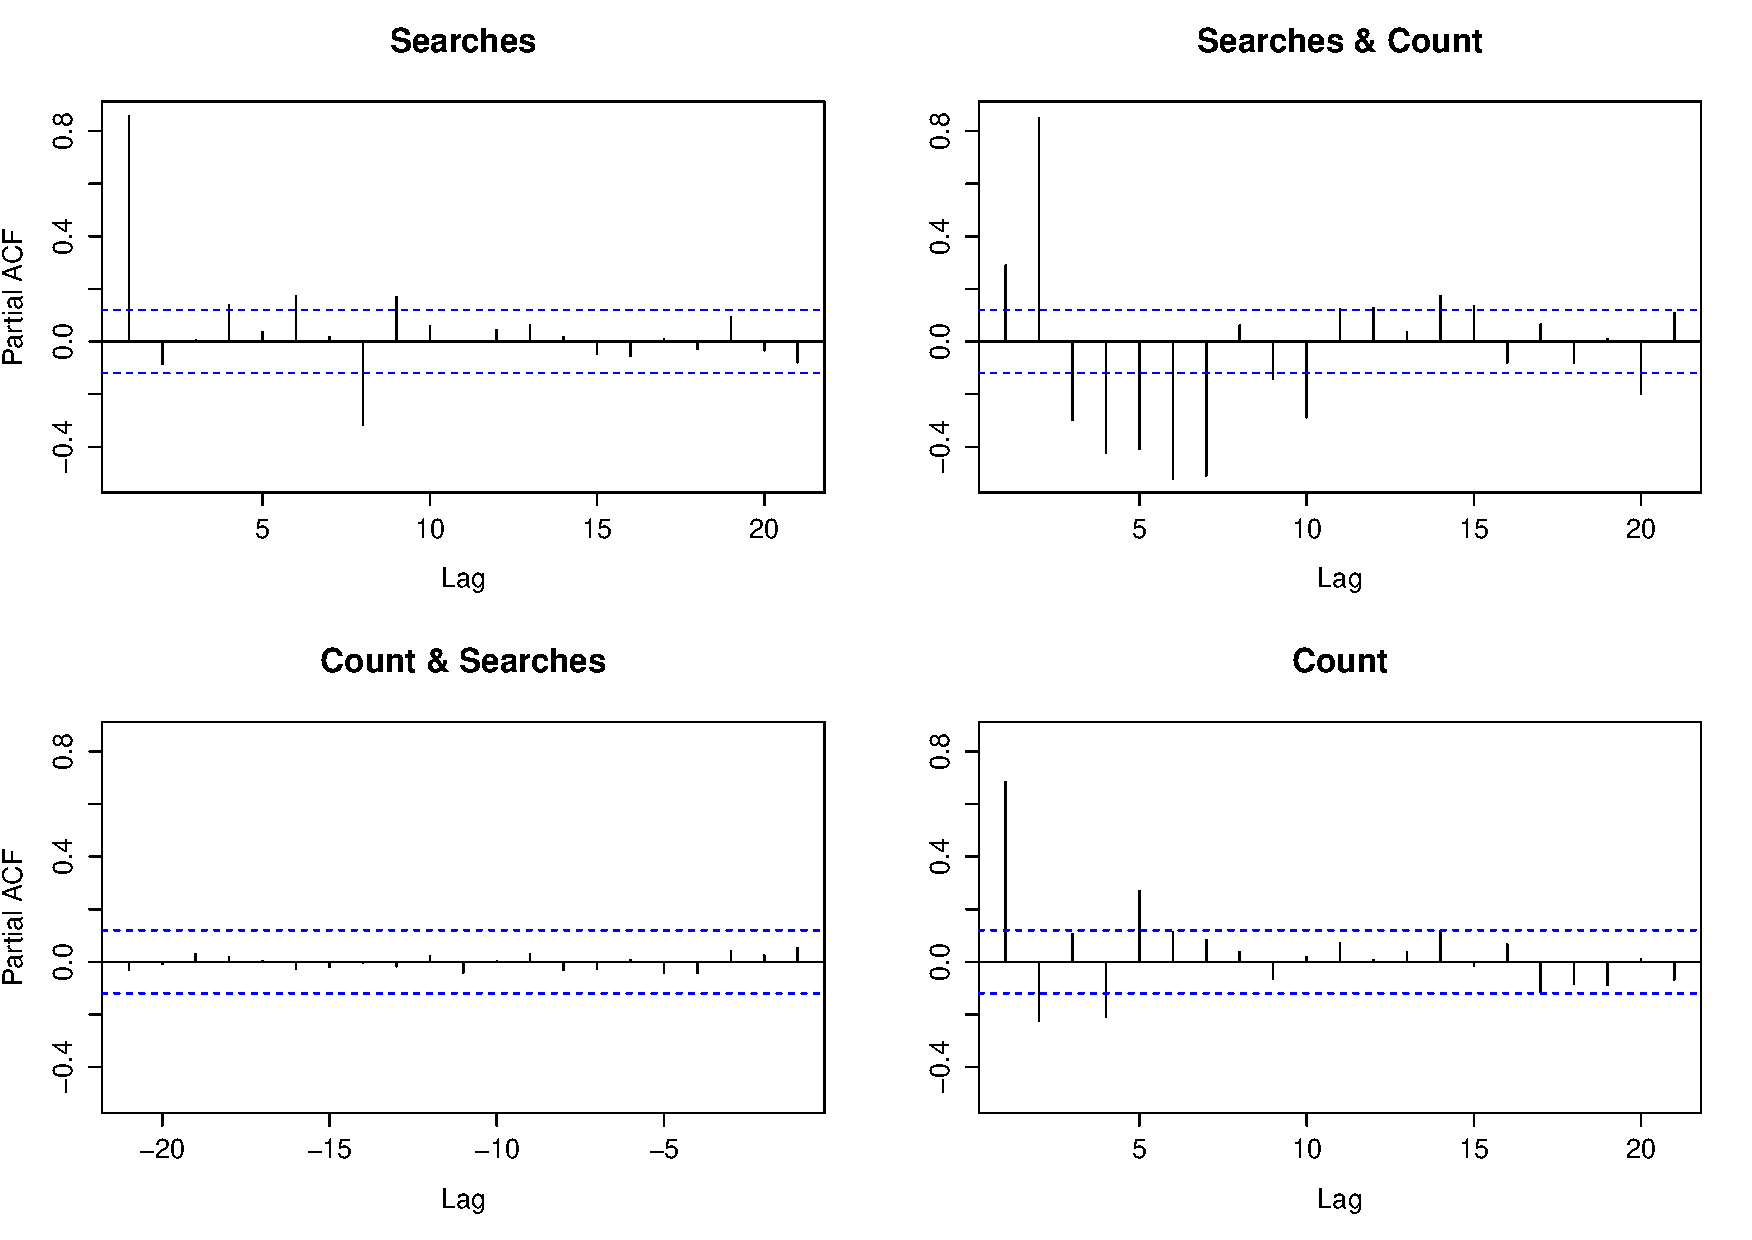
\includegraphics[width=\textwidth]{partial_autocorellation}
\end{center}
\caption{Partial autocorrelations for the data set. The blue dotted line is the 95\% confidence level, anything above is statistically significant.}
\label{megacor}
\end{figure}


\subsection{auto.arima}

Using the autocorrelation plots is a perfectly reasonable way of finding your parameters. However, since we have no previous experience in using them it was better to use the auto.arima function. It finds the optimal parameters for your data using Maximum Likelihood and it yields the model ready to use. 

For our case the auto fit yielded that the best order for Sochi in particular is 4, 1, 5. That means that Sochi is a non-stationary time series ( does not have a constant mean and variance) and the ARIMA is an autoregression of the 4th order, moving average of the 5th order and differencing of 1st order to "stationarise" the time series. The fact that some of the series are stationary, while others are not only increases the utility of having this auto fit, since it cannot be guaranteed that a single fit all solution would work on a destination basis. 

Forecasting with the fitted model is very easy as well. R is excellent for time series forecasting and with 2 easy commands one has forecasts without any problem. As you can see in Figure \ref{arima-forecast} the forecast has kept the seasonality of the time series. We will explain more in the Results chapter, where there will be a discussion.

\begin{figure}[]
\begin{center}
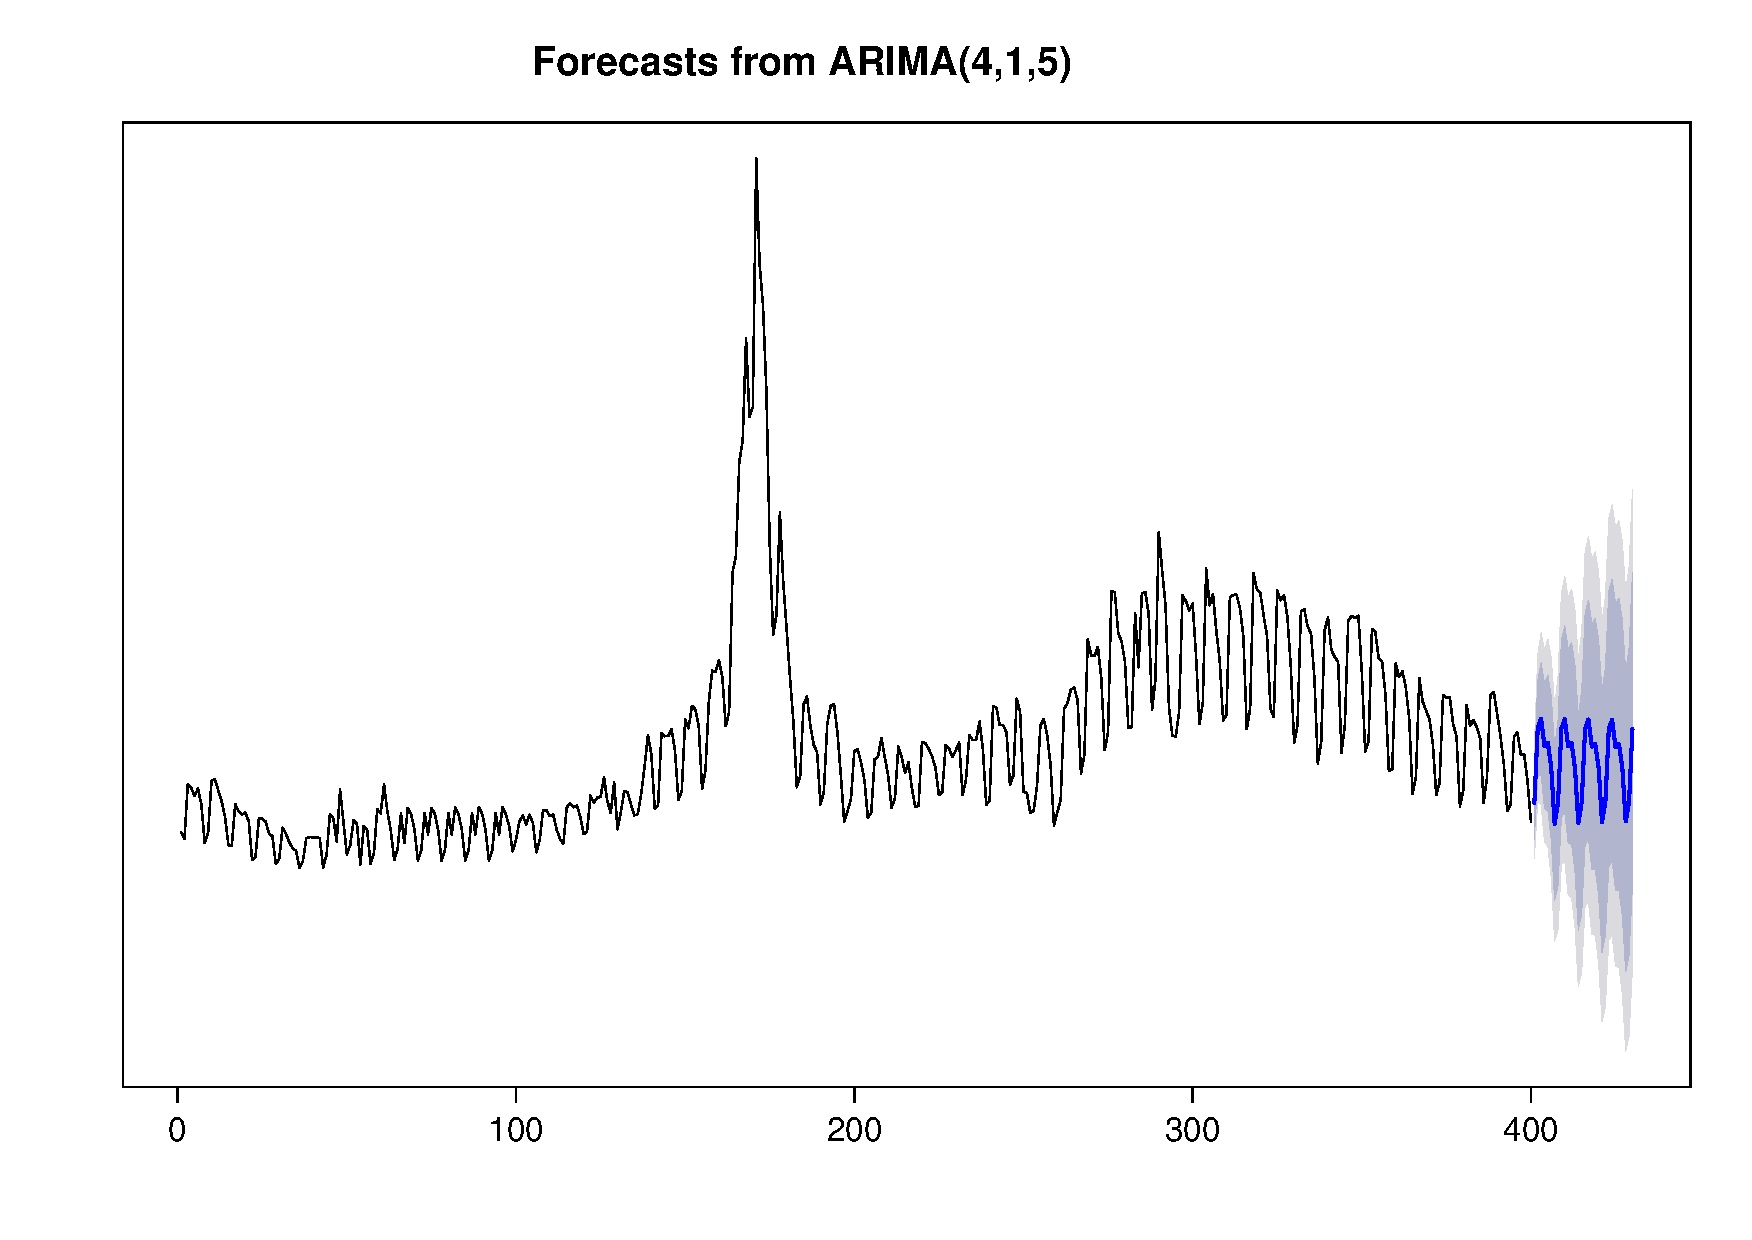
\includegraphics[width=\textwidth]{arima_forecast}
\end{center}
\caption{ARIMA Forecast}
\label{arima-forecast}
\end{figure}

\section{Conclusion}

In this chapter we have given an overview of the models used and a justifications of why they were used. In Chapter 5 we will present the results, discuss the results and show which model performed best.

In the next chapter we follow with an overview of the algorithm used for finding change points.        

\chapter{Methodology}
%explain more about Twitter

As the reader is now aware this is the second phase of this MInf project. All the heavy lifting in terms of data collection, processing and cleaning has been done in the first part and we have not changed it at all, because there was no need to do so. The system developed as part of Phase 1 was continuously used for all the tasks end-to-end and it is described in a bit more detail in Chapter 2. 

Last year's work produced some interesting results and did improve forecasts by 5\%, however we would not be very wrong to say that those models were something that was used as a black-box. Of course, the author had an understanding of how they worked, but we did not work towards one of the goals we set out - to try and find the times where something odd is happening.

In order to do that we had to depart from the programmers mindset of complete automation - developing the tools that we can chain together and get everything done easily. Instead we had to dig deeper into the data, find a few destinations that we knew something - be it an event of significant or something else, focus on that and develop and algorithm that will find those change points based on past data and Twitter and alert if something is happening and then of course, if one needs to use an automated tool the algorithm could be easily integrated into the current system.

Therefore it should not come as a surprise that we decided to focus more on the modelling side. Because of the availability of the data and its volumes we have entered into this mentality where you just throw the data at some models and see what happens. That of course means that we can do quite a lot of things and of course eventually find what works, but also because of not knowing the models, we are wasting time trying things that do not go well together. 

First and foremost, this section will be concerned predominantly with change point detection. There will be an introduction into the topic with some overview of different research and how this ties together with the problem we have set out to solve. Afterwards we will go through the different tools that we have used, why they did not work as we have expected and the algorithm that we implement ourselves. 


\section{Introduction to Change Point Detection}


Change Point Detection\footnote{\url{http://en.wikipedia.org/wiki/Change_detection}} or as it is also known change detection is a way of identifying times when the underlying probability distribution of a stochastic process or time series changes - before the change point data is drawn from one distribution, after the change point, data is drawn from a different distribution. The problem can be broken down into a few sub-problems:
\begin{enumerate}
\item Has a change occurred or not?
\item If yes, how many changes have happened and at what times?
\end{enumerate}

There are specific applications like step detection - finding step changes in time series - and edge detection - which deals with digital images - who are concerned with changes in the mean, variance, correlation or spectral density of the process/time series. As a sub discipline change detection also includes the detection and flagging up of anomalous behaviour, which is also knows as anomaly detection. 

Change point detection itself is extremely useful for many different fields. We have listed two examples above, which have very specific applications - like detecting edges in pictures. However just step detection, which is a sub discipline of change point detection can have many different applications:
\begin{itemize}
\item It is commonly used in exploration geophysics to where it is used to segment well logs into different stratigraphic zones;
\item Used in genetics to separate micro-array data into different copy-number regimes;
\item Also used in biophysics to detect state transitions.
\end{itemize}
 

Online algorithms will usually run at the same time as the process or time series or events they are monitoring and they will be taking in and processing each and every data point as soon as it becomes available. It is also important to note that the processing of the this data point should be complete before the next data point point arrives of the real-time constraints. Offline algorithms on the other hand will go through the data set in its entirety, evaluate everything and output when done, because there are no real-time constraints.

Therefore in most cases we can generalise that "online" can simply mean that the algorithm is fast enough to keep up with the data stream. In other cases it means that it is incremental - meaning that every time a new data point arrives the algorithm could easily perform an update of the required statistic instead of precomputing everything from scratch (run in O(1) time). Those type of algorithms are particularly appealing nowadays in a variety of places - embedded processing or real time analytics, where processing power is  premium or being able to get the outcome as soon as possible is essential. 

"Online" and "Offline" are simply used to describe the problem formulation and how the algorithm is expected to work rather than the algorithm. In the online scenario we would be striving to minimise the time to detection, while also decreasing the rate of false alarms. On the other hand in offline detection, we would not have the pressure to do it as soon as possible, since we will be able to fine tune the algorithm on the whole sequence and the criteria there would be to maximise the sensitivity of the algorithm - the number of actual change points detected - and avoiding false positives.

Adaptive Filtering and Change Detection \cite{Gustaf} by Fredrik Gustafson is probably the best book on the topic. The author outlines various ways to solve the problems:
\begin{enumerate}
\item The standard changes in the mean and variance - described in Section \ref{sec:basic};
\item AR \& ARX - a new algorithm using ARX and ARIMA described in Section \ref{sec:novel};
\item Regression models;
\item State space models;
\item Non-linear models.
\end{enumerate}

In the following sections of this chapters I will explore some of the options who were available off the shelf and discuss whether they are a suitable candidate for the task. 

\section{Change Point Detection off the shelf}

\subsection{Changes in the mean}
\label{sec:basic}

Perhaps the simples of all models are the changes in the mean, variance and the one that combines both. The \textbf{changepoint}\footnote{\url{http://cran.r-project.org/web/packages/changepoint/changepoint.pdf}} package in \textbf{R} fortunately had those methods all easily available, so we could easily carry out the testing of the different models without having the overhead of implementing every single method ourselves. 

Running the change point detection was trivial with various configurations, however one thing was apparent. It was segmenting the data at different partitions and while the boundaries of those partitions are arguably change points it is just additional overhear of trying to get get it to work as we would like. In Figure \ref{mean-best-output} we present how the changes in the mean model simply segments. We have the option to use 4 different methods for finding the change points:
\begin{enumerate}
\item AMOC - At most one change - the default option. Basically here we only try to find the single change point in the data. In our case that is not useful, since we are trying to find whether change points exist in the data, so we are not certain of their number. 
\item BinSeg - the most popular approach to identifying change point. It works on a principle rather simple to recursion or merge sort - you apply a single change point test statistic to the entire data set. If a change point is identified, then you split it into 2 locations. Then you repeat it on the new datasets - before and after the split. If you find any new ones, you split again and continue splitting until nothing new has been identified. The algorithm is approximate.
\item SegNeigh - the algorithm works by minimising (4.1) by using a dynamic programming technique to obtain the optimal solution for m+1 change points and split the data into $m$ ``neighbourhoods".
\begin{equation}
\sum_{i=1}^{m+1} [ C(y_{(\tau_{i-1}+1):\tau+{i})}] + \beta f(m) 
\end{equation}
where where C is a cost function for a segment e.g., negative log-likelihood, $\beta*f(m)$ is a penalty to guard against over fitting and y is the ordered time series.
\item PELT - \textbf{P}runed \textbf{E}xact \textbf{L}inear \textbf{T}ime, which is a dynamic solution to the segmentation of data. Typically faster than others, because of its dynamic nature. It is very similar to SegNeigh, because it provides an exact solution, but because of the pruning it can be shown to be much much faster than its counterpart. 
\end{enumerate}


\begin{figure}[]
\begin{center}
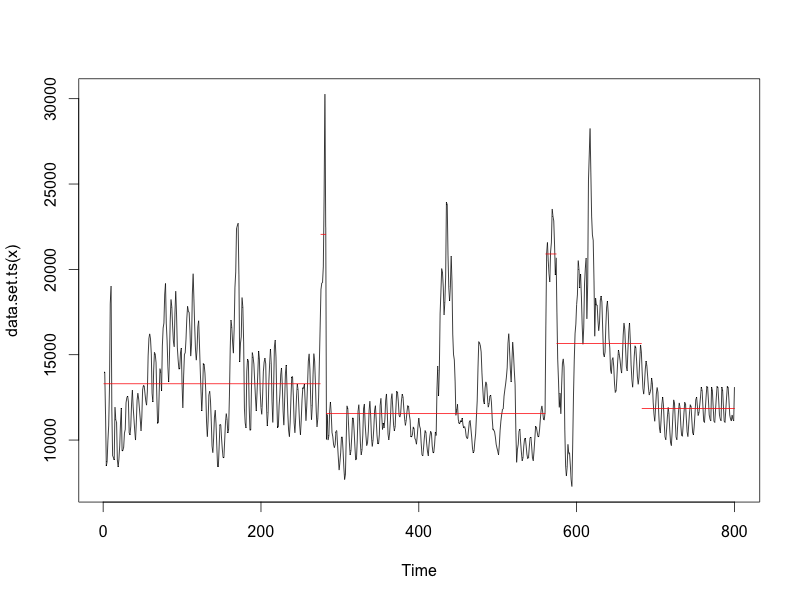
\includegraphics[width=0.9\textwidth]{fictional_town_mean}
\end{center}
\caption{Change points determined by changes in the mean on generated data. Red lines denote the different segments. Change points are the ends of the lines.}
\label{mean-best-output}
\end{figure}
\begin{figure}[]
\begin{center}
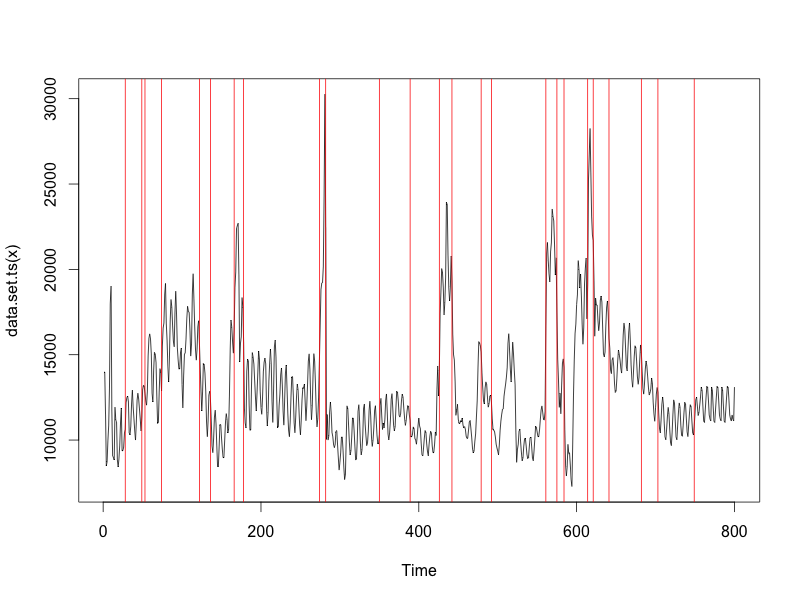
\includegraphics[width=0.9\textwidth]{changes_in_var}
\end{center}
\caption{Change points determined by changes in the variance on generated data. Red lines denote the different change points.}
\label{var-best-output}
\end{figure}


Since the methods are easily available, we could try all of them one by one, however none of them really yielded anything that we could use as a change point, simply to the fact that it is a useless output for us.  You can see in Figure \ref{mean-best-output} how the output generate from changes in the mean with a \textbf{BinSeg} search algorithm on a generated data set. Even though the ends of the red lines, which are the change points in this case, do indeed align with some of the abrupt changes in the profile of the time series to this fictional place, we can see that quite a lot of the ones that are visible - especially in the second segment are not flagged up. PELT on the other hand bizarrely enough flagged every single point as a change point, while SegNeigh could not finish the computation for the example data set we used for comparison. 


\subsection{Changes in the variance}

The next change point detection method we will try is changes in the variance. In Figure \ref{pelt-meanvar} we have shown the output from running changes in the variance with the \textbf{PELT} search algorithm on the same generated data set as above. Unlike the previous method, with this one we have the complete opposite of the problem, here we are alerting simply far too often, even for a single change in profile we are alerting multiple times, thus increasing the rates of False Positives quite a bit. 
 \textbf{SegNeigh} and  \textbf{BinSeg} on the other hand returned too few change points, which was not sufficient. 


\subsection{Changes in mean and variance}

The final supported way of finding change points in the package was by finding changes in the mean and the variance at the same time. Needless to say the results were not massively different from before. As we can see in Figure \ref{pelt-meanvar}, PELT produces far too many, while in Figure \ref{meanvar-binseg} we can see that BinSeg does the complete opposite and splits the data in far too few regions. 

\begin{figure}[h!]
\begin{center}
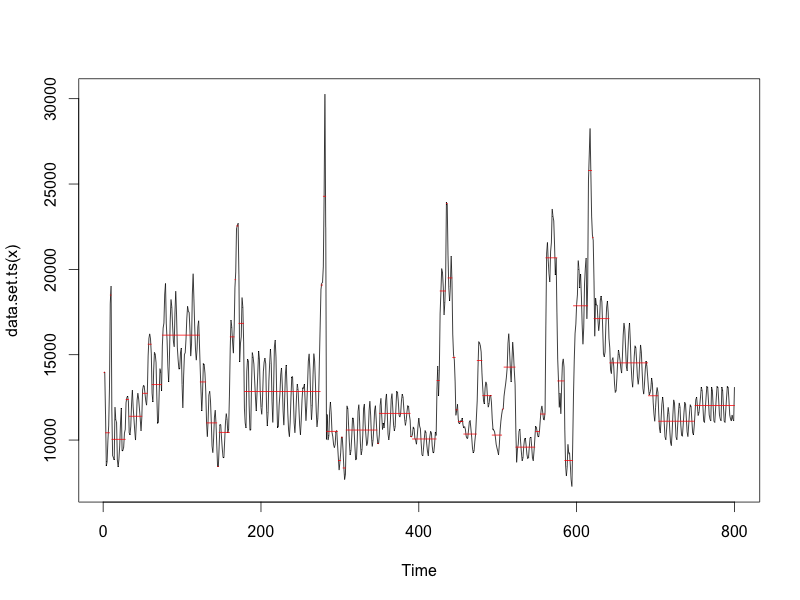
\includegraphics[width=\textwidth]{meanvar_pelt}
\end{center}
\caption{Change points determined with changes in mean and variance with PELT.}
\label{pelt-meanvar}
\end{figure}
\begin{figure}[h!]
\begin{center}
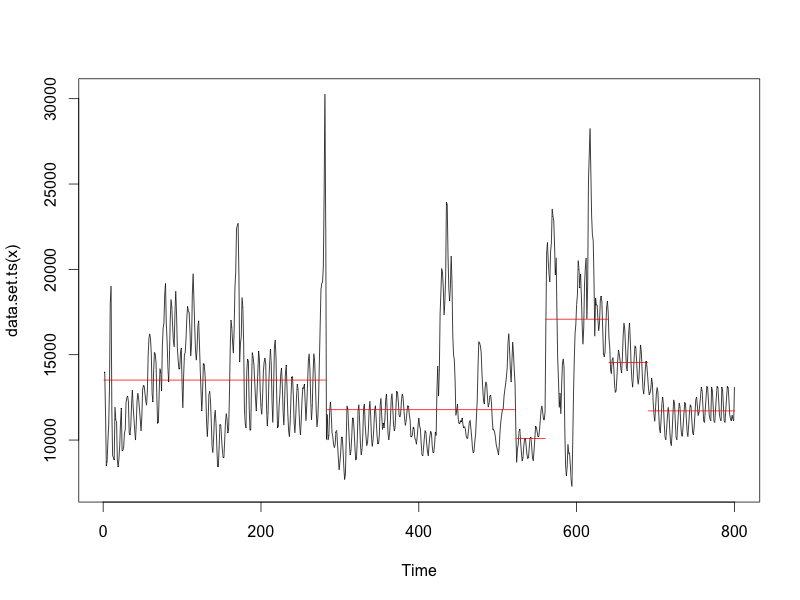
\includegraphics[width=\textwidth]{meanvar_binset}
\end{center}
\caption{Change points determined with changes in mean and variance with BinSeg.}
\label{meanvar-binseg}
\end{figure}

\newpage
\subsection{Conclusions}

In this subsection, we have explored the \textbf{changepoint} and \textbf{bcp} packages and whether an off the shelf solution could be used. However we believe that for the following reasons it is not suitable:
\begin{enumerate}
\item Either overestimates or underestimates the number of change points. 
\item For the best results, we would need to know the number of change points otherwise the results look odd.
\item The time spend tweaking the parameters could be spend implementing and using a custom tailored algorithm that will predict change points in the way that they are required for events. 
\end{enumerate}

For all of those reasons we decided that the time we could have spend tweaking this would be better utilised by implementing our own search algorithm. 


\section{Bayesian Change Point Detection}

PLACEHOLDER

\begin{figure}[]
\begin{center}
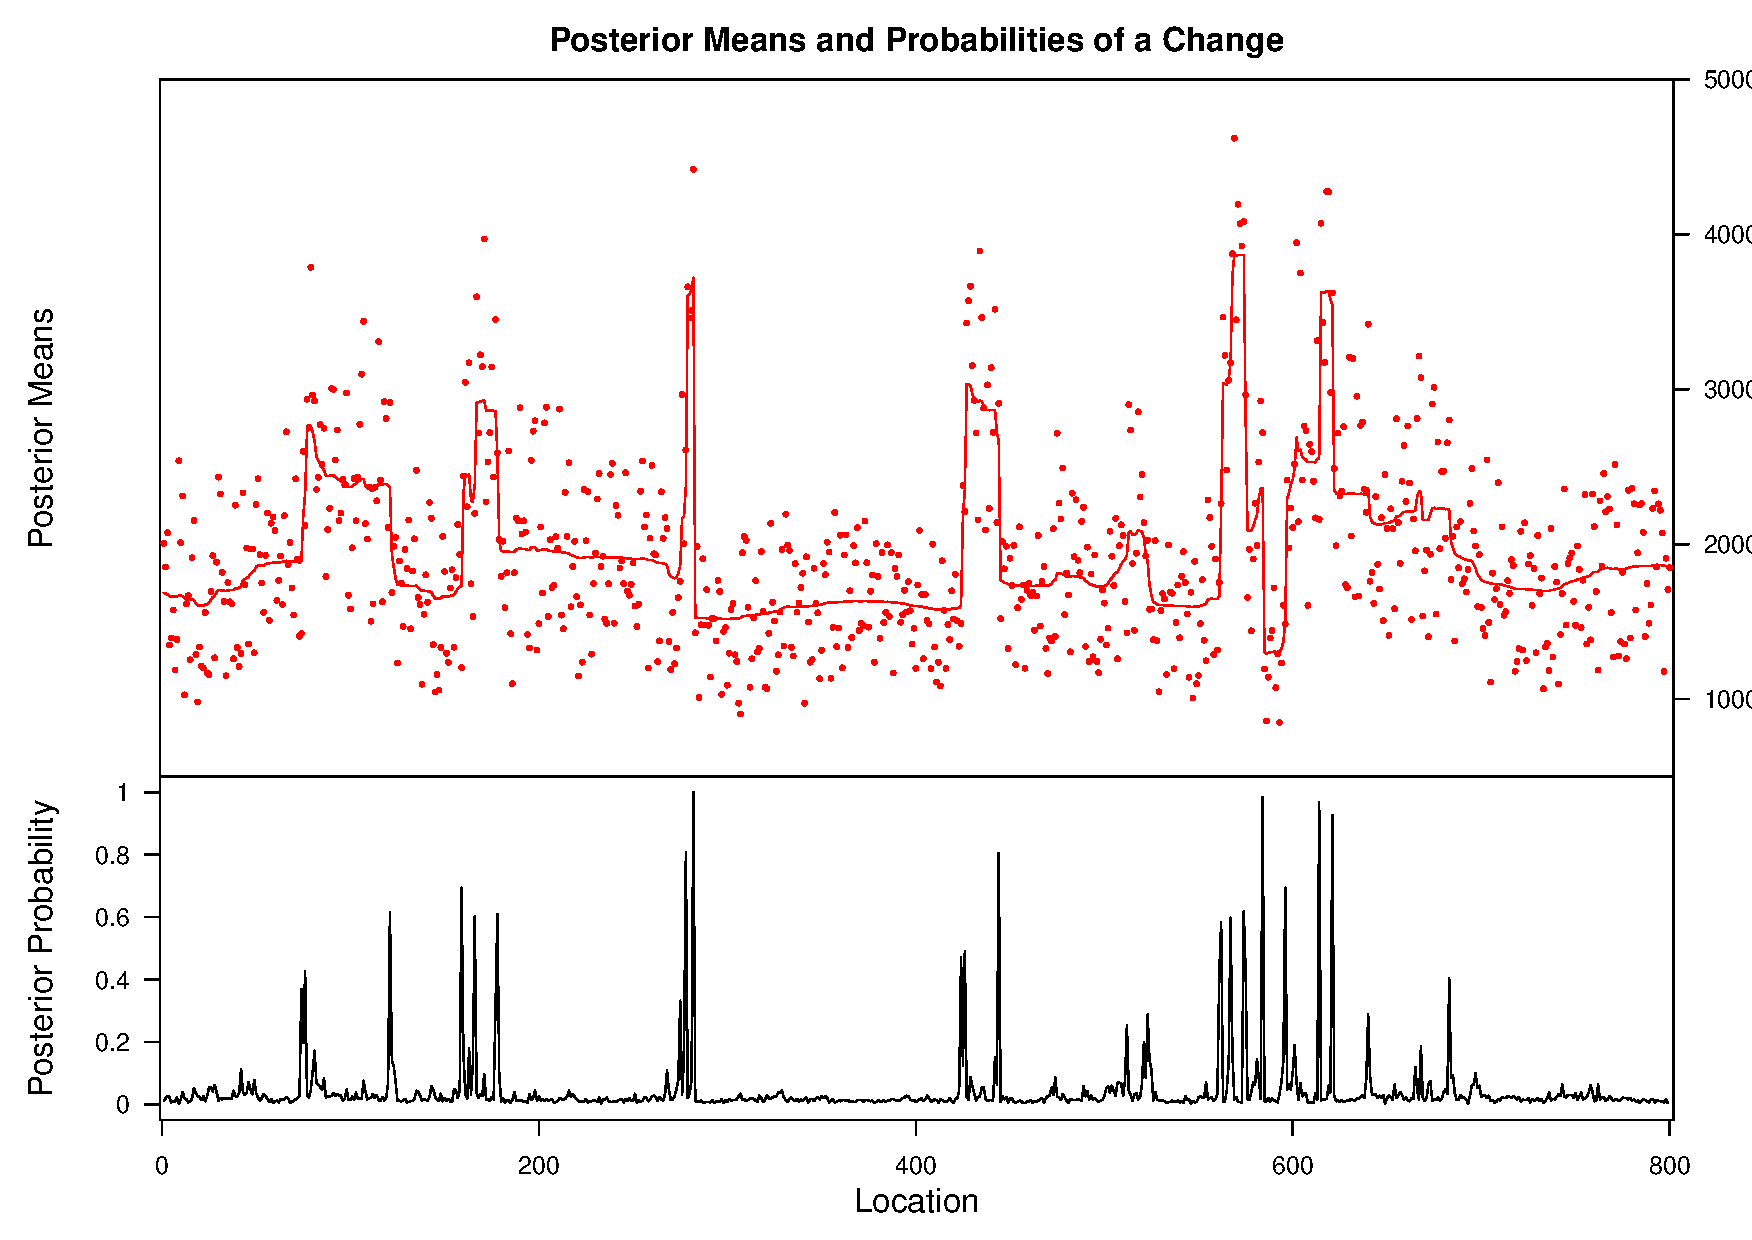
\includegraphics[width=\textwidth]{bcp}
\end{center}
\caption{Online bayesian change point}
\label{bcp}
\end{figure}


\newpage
\section{Novel method using ARIMA}
\label{sec:novel}

Since none of the packages that we explored produced results in a way or form that we found suitable we had to go down the path of implementing our own algorithm that would alert when  big event has happened and therefore there is a spike or other change in the profile of a time series that does not fall within the normal seasonality. 

We created 2 versions of the algorithm - one that is offline and an online version as well. The offline one was used mostly for hypothesis evaluation - to see whether the idea would would and then when we saw that it does work indeed we decided to progress with the online one and carry out the extensive tests with it.


\subsection{Algorithm}

The algorithm itself is rather simple. We take 4 weeks worth of data to train the model, which in our case is an ARIMA model. 

The offline version of the algorithm works the following way - we accumulate a statistic of all the residuals and then we iterate for every point $t$ for $t$ in $[min:N]$, where $N$ is the number of data points and  $min$ is the starting point for the algorithm. For every $t$:
\begin{enumerate}
\item Fit an ARIMA for the data $1:t-1$;
\item Use the ARIMA to predict $\hat{y}_t$; 
\item Store $\hat{y}_t  - y_t$.
\end{enumerate}

Then we are doing a second pass over the data and if:
\begin{equation}
\hat{y}_t  - y_t> \mu + 2*\sigma || \hat{y}_t  - y_t < \mu - 2*\sigma
\end{equation}
then we have a change point and we alert. That of course means that we assume that the residual distribution is Gaussian, but more on that in the next subsection. Just as a note for the first 2-3 months of running the data, we use $3*\sigma$, because of the fact that there is simply too little data in the beginning. 

The online version is similar, but we incrementally update the mean and standard deviation \footnote{\url{http://en.wikipedia.org/wiki/Algorithms\_for\_calculating\_variance#Online\_algorithm}} and we do not do a second pass over the data. 

\subsection{Offline version}

The offline version was not ultimately the version that we used in our results, but it was very important, because it allowed us to explore the data, see what the residual distributions looks like and ultimately validate the hypothesis that an algorithm would work. The results produced were inline with our expectations.  

In the offline version it was very important to confirm first of all that the residuals distributions comes from a normal distribution because that had massive implications of the online version:
\begin{enumerate}
\item Incrementally updating the mean and standard deviation of a gaussian is very easy;
\item Detecting the outliers with a normal is easy again;
\end{enumerate}

Therefore after the first pass over the data we accumulated all the residuals and plotted their density distribution. For Sochi this  the error density (Figure \ref{error-density}) looks spectacularly like a gaussian, while the absolute error density (Figure \ref{abs-error-density}) not so much. 

\begin{figure}[]
\begin{center}
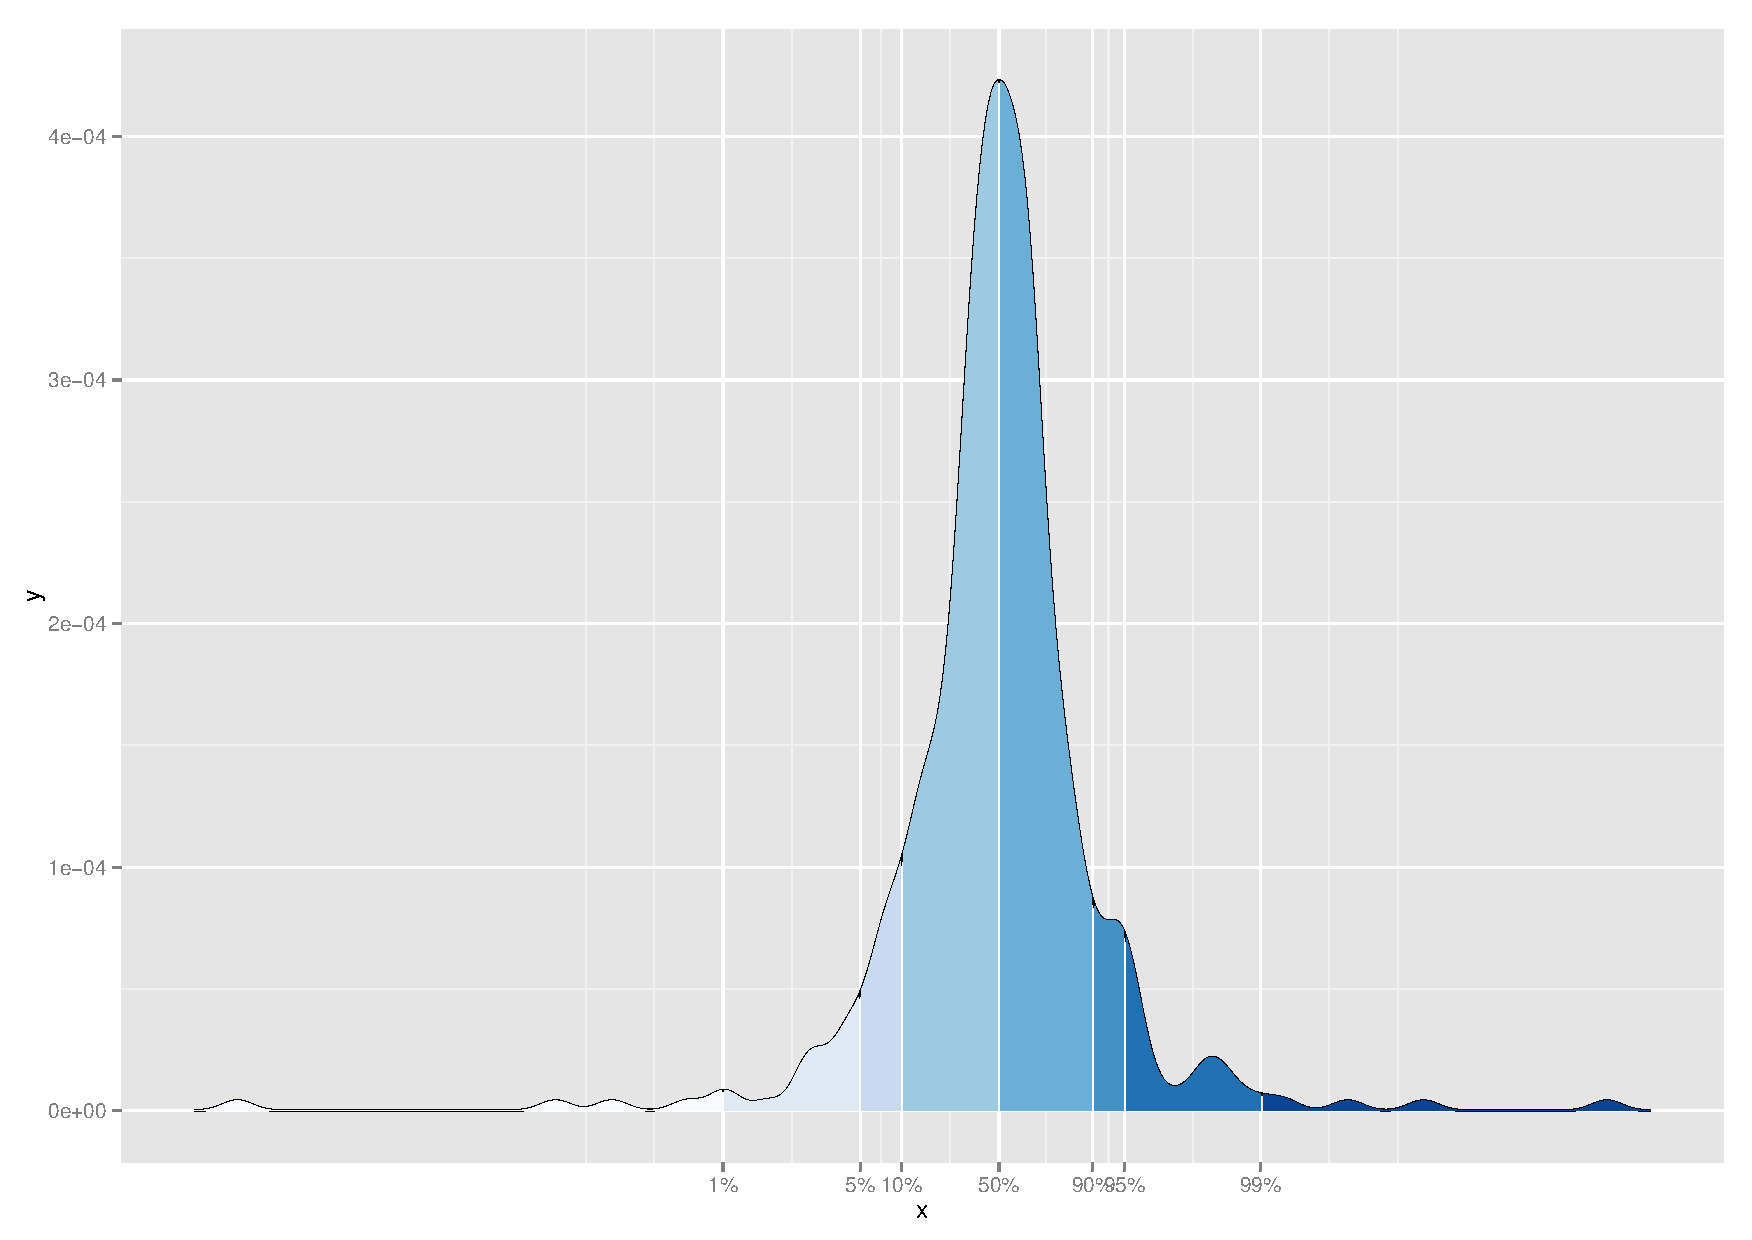
\includegraphics[width=\textwidth]{percentiles}
\end{center}
\caption{Plot of error density.}
\label{error-density}
\end{figure}
\begin{figure}[]
\begin{center}
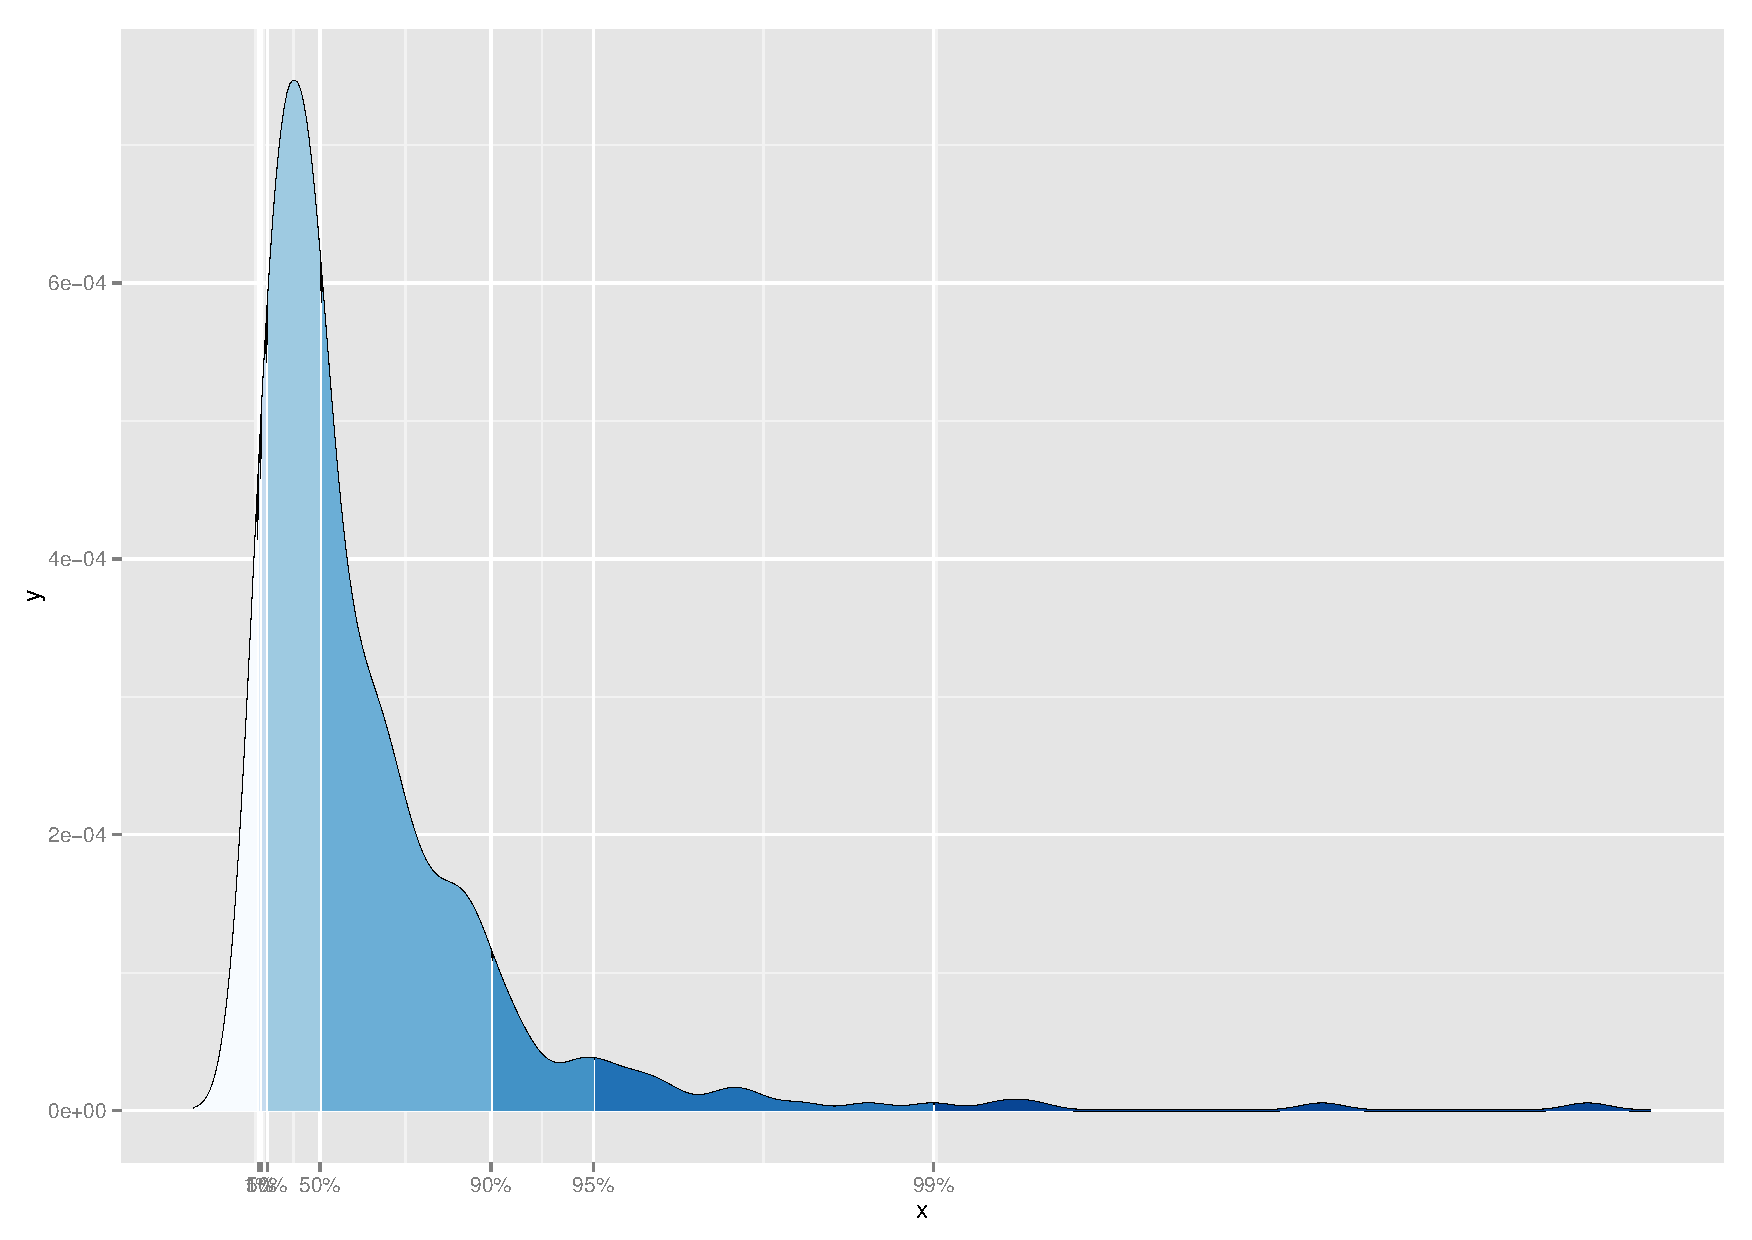
\includegraphics[width=\textwidth]{error_plot}
\end{center}
\caption{Plot of absolute error density.}
\label{abs-error-density}
\end{figure}

Now that we have done the residual density and it does look like a Gaussian we had to continue with developing the 2nd pass where we will be making the decisions whether something is a change point or not. Of course we want to be taking only the anomalies - times when the prediction is wildly overestimating or underestimating the number of flights searches. When it is doing either it basically means that something dramatically different has happened. 


Sochi is our favourite go-to place to work on, purely because we know that something very big happened there - the Winter 2014 Olympic Games. Because of that there is one massive spike exactly at the time of the games, which we can see in Figure \ref{offline-method}. The number of change points alerted was drastically reduced from the off the shelf packages, since this particular implementation has been tailored precisely for this use case. The most amazing fact at least for us the fact that the systems works exactly as intended which flags up the massive peak during the Olympics. 

\begin{figure}[h!]
\begin{center}
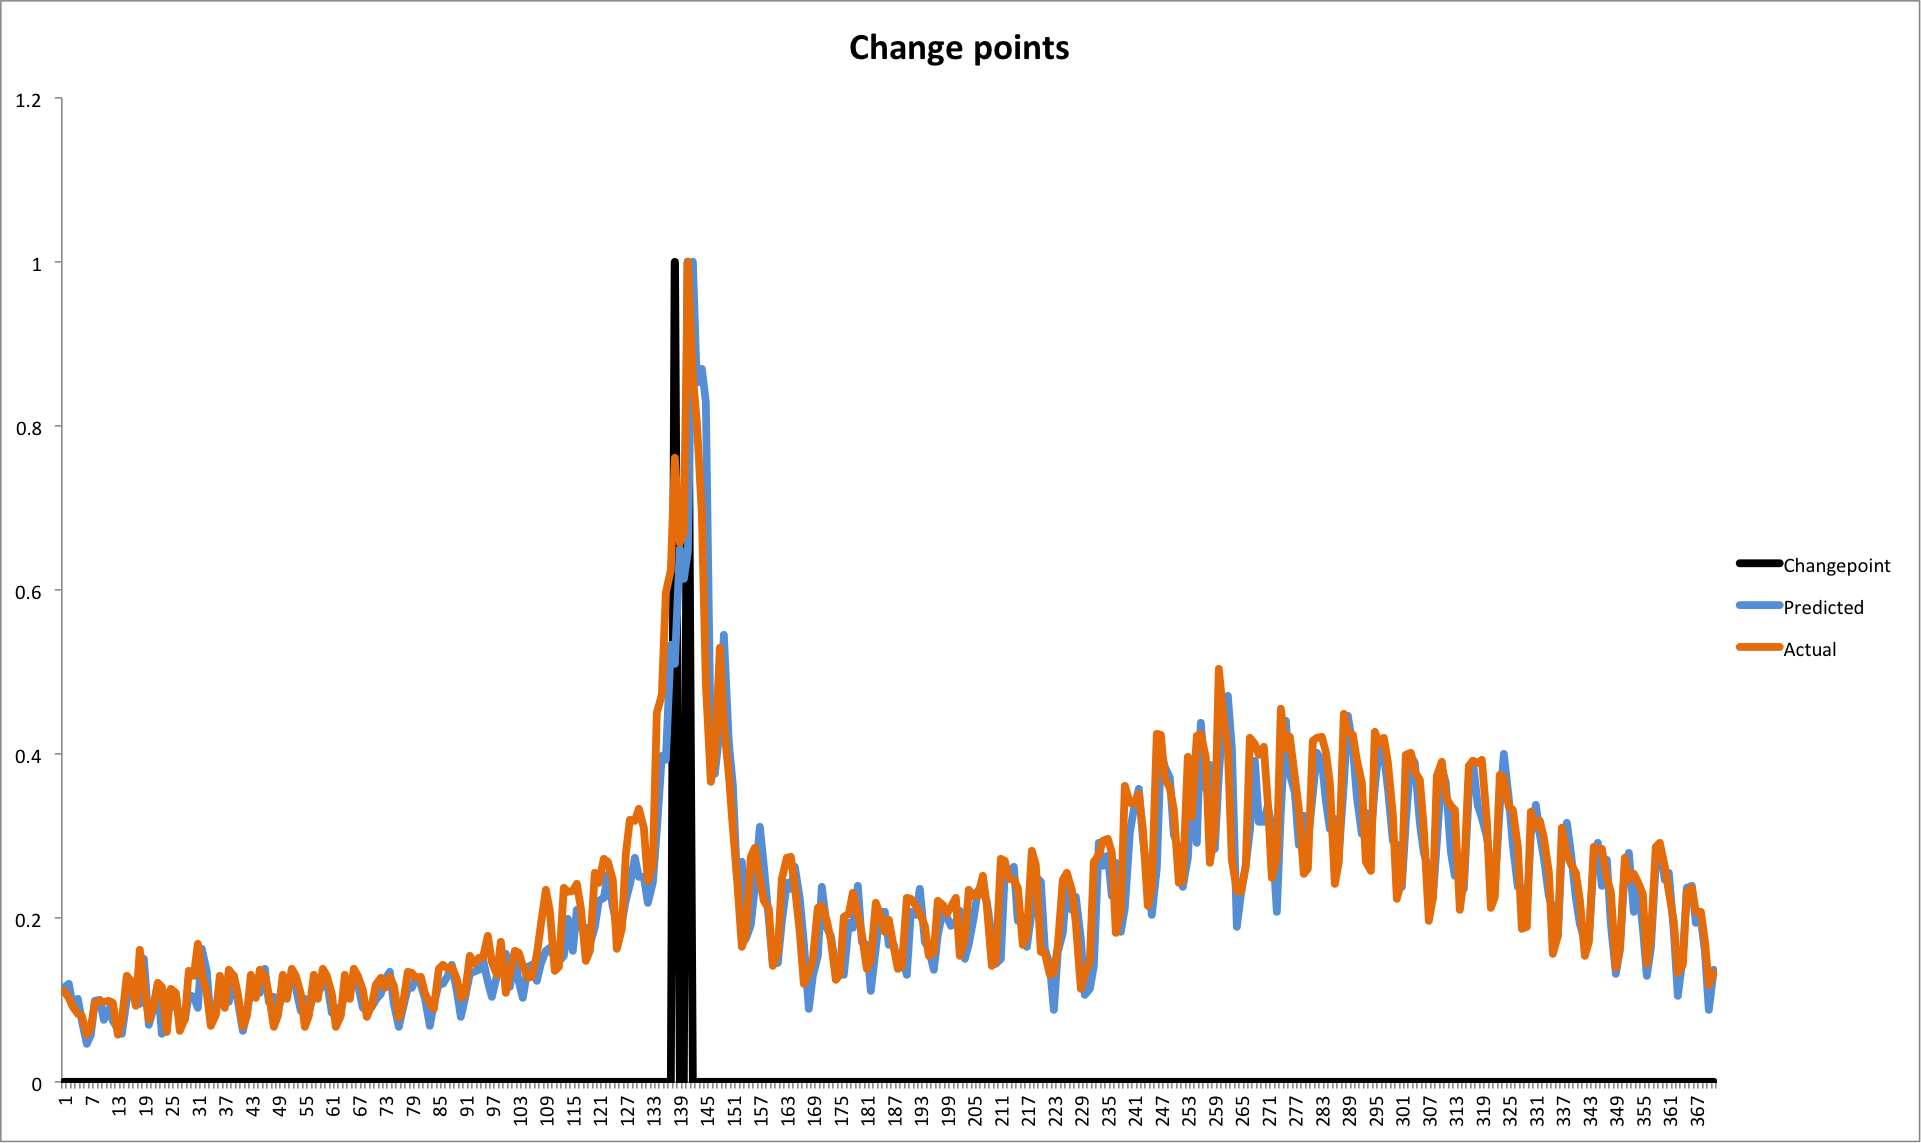
\includegraphics[width=\textwidth]{Changepoint_99}
\end{center}
\caption{Change points determined as per the second method.The actual values are orange, the light blue is the ARIMA prediction and black is the binary change point flag as per the algorithm.}
\label{offline-method}
\end{figure}


That means that due to that particular event we can easily "smoke test"\footnote{Perform a very quick test} to see whether the model would hold up to the most basic of tests, which in our case was whether it would detect the massive spike around the Winter olympics. and it did as we can see! That was very encouraging, because it meant that it was doing the kind of change point detection we want - around big events, that disproportionately affect flight searches demand in a way that does not fit the current models. 

As a conclusion we would like to say that the offline performed very well indeed, but most importantly the way we interned it to. Since the offline version has confirmed that this can be done, now it was time to explore the online version, with the hope that the online version will speed things up since it will require only one pass over the data. 


\newpage
\subsection{Online}

As mentioned in the previous subsection the results were promising, since the offline version worked exactly as intended. 
Now it was time to make it work online. 

In order to do that, first of all, we had to get rid of the accumulation of the residual statistic and update the mean and the standard deviation incrementally. If we had it done the way it currently worked it would have meant that for every data point we would have to do a pass over the data, to get all the at a points and compute the running stats from that. 

Instead, I used an algorithm that has been published by Donald Knuth\footnote{\url{http://en.wikipedia.org/wiki/Algorithms\_for\_calculating\_variance#Online\_algorithm}}, who himself cites Wetford\cite{online-mean-and-var}. 



\begin{figure}[h!]
\begin{center}
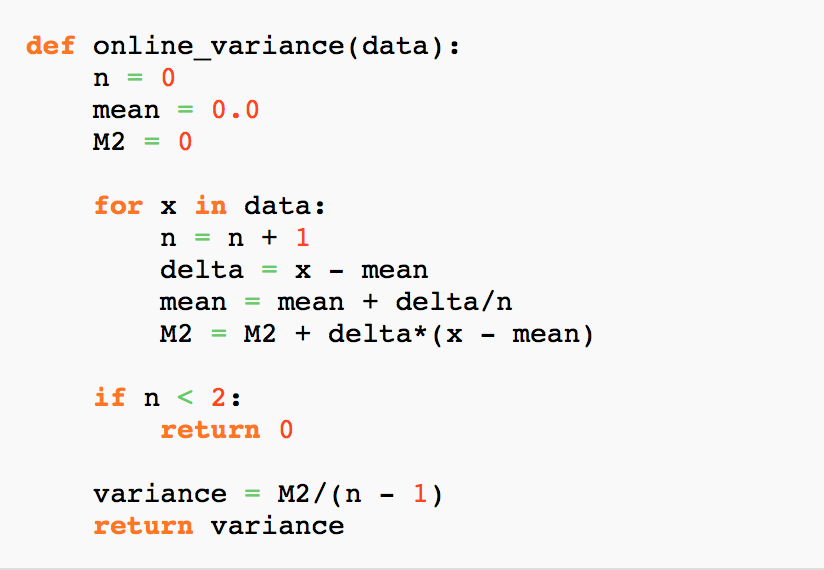
\includegraphics[width=\textwidth]{online_algo}
\end{center}
\caption{Algorithm for incrementally updating the mean and the variance. Standard deviation is obtained by simply taking $\sqrt{\sigma^2}$ or in this case $\sqrt{\frac{M2}{(n-1)}}$ as it is denoted in the code}
\label{mean-formula}
\end{figure}


It is a rather simple algorithm, but it is been proven to work and the computation overhead is minimal in comparison to trawling through all the data points before that to find the mean and variation, especially since it can now be computed on the fly. 

Another big advantages was also the fact that with the online version, we could carry out tests much faster than with the offline one, which in turn meant that acquiring data was much faster. 

In Figure \ref{NK} you can see the results from the algorithm for North Korea. The change point detection is visible with the purple squares at $x=1$. They do align with some of the changes in behaviour - such as the first big spike around $\tau = 80$, the big jump at $\tau = 160$ ad massive increase in searches at $\tau = 390$, however there are still some of those peaks that are missed. 

\begin{figure}[h!]
\begin{center}
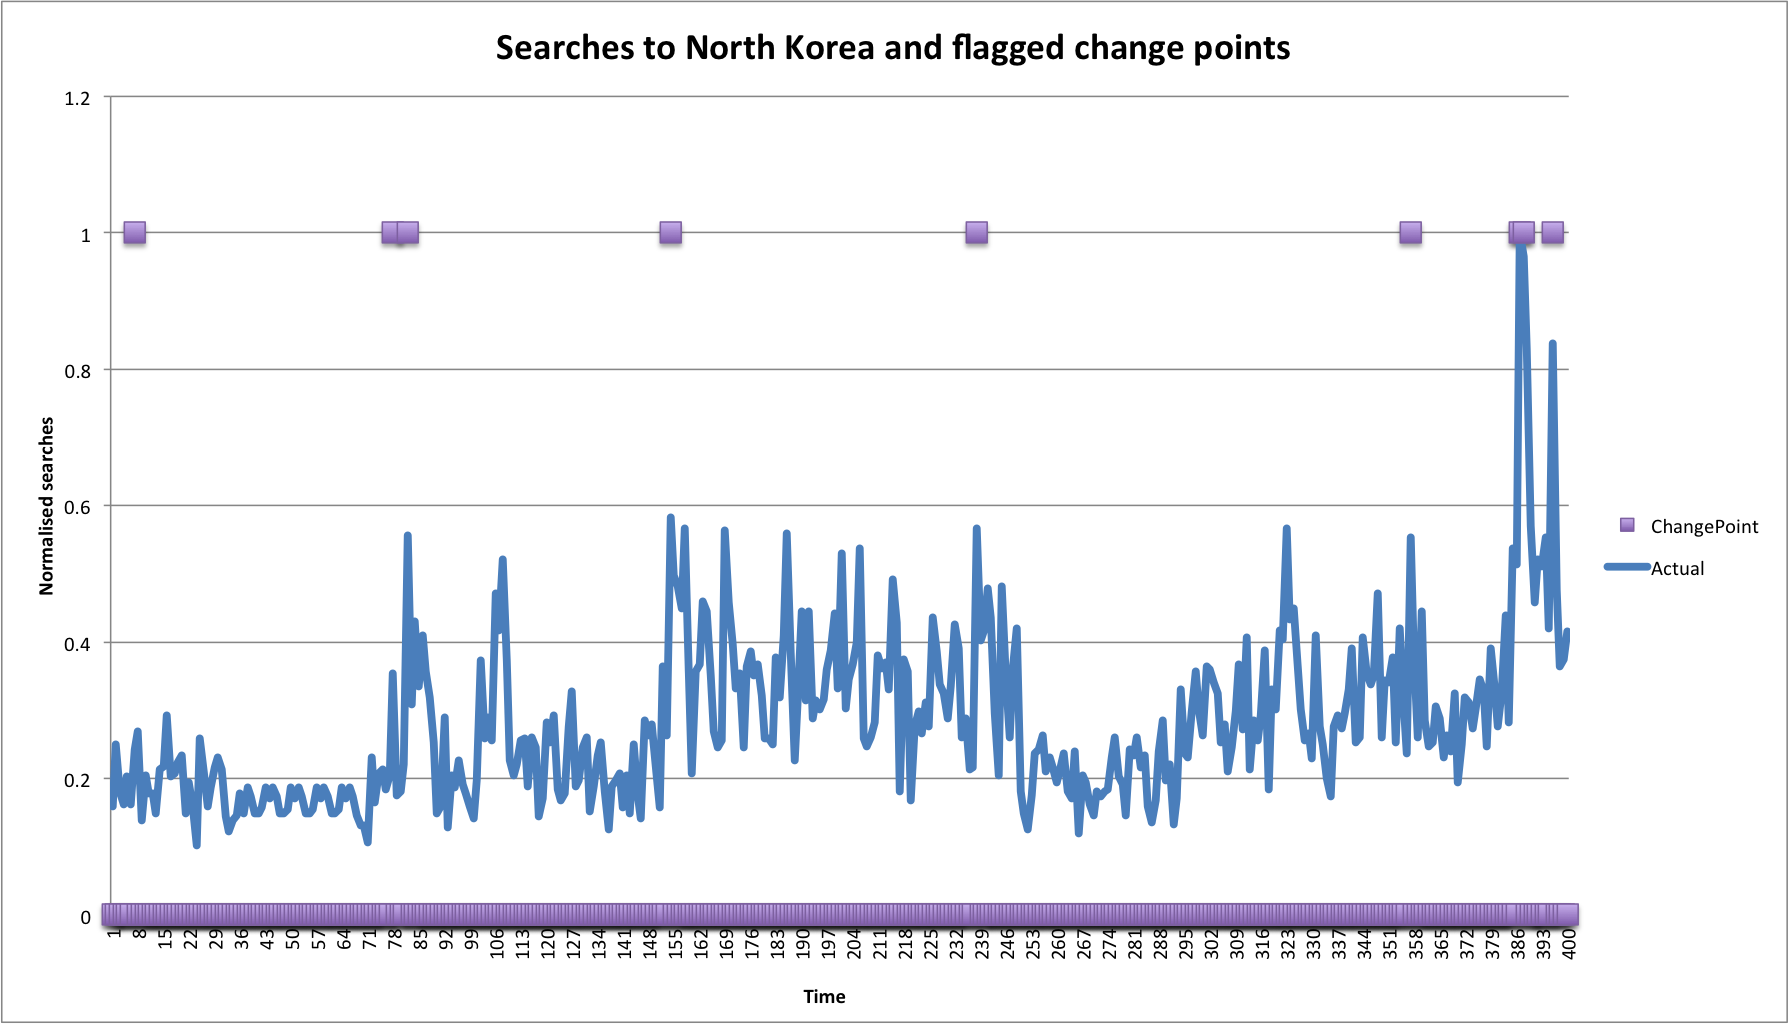
\includegraphics[width=\textwidth]{NK}
\end{center}
\caption{Output for NK. The purples squares is the ChangePoint binary flag - 0/1 and the blue line is the normalised number of searches}
\label{NK}
\end{figure}


The results of the online algorithm and how it impacted the search prediction will be discussed in more depth in Chapter 5. 

\newpage
\section{Conclusions}

In this Chapter we have given an overview of the different algorithm and methods that we have used in this work. Here we shall summarise our findings in a bullet-point form.

\begin{itemize}
\item The simple models (changes in mean, variance, mean and variance) did not yield the kind of results we would want, therefore they will not be taken any further for the testing. 
\item The Bayesian Change Point Detection worked really well off the shell, so we will try to incorporate it into our tests for the actual systems. 
\item The novel algorithm using the ARIMA worked really well, and it will be certainly included into the final test, simply because it is tailored for the task. 
\end{itemize}


\chapter{Results}

In this section we will present the results from this work and discuss them. We have split this chapter into X sections:
\begin{enumerate}
\item The test set - explanation and examples of the test set
\item ARIMA vs L4F - comparison of ARIMA and Last 4 Friday. 
\item Change point detection - analysis of the change point detection results
\item ARIMA + change points factored in and how it performs.
\end{enumerate}

\section{The test set}

For this particular testing, rather than to test across the full set of 1600 cities and countries, we have decided to instead test on a smaller scale, since the tests done here required more manual work to get done. We manually set out to find some places that have an interesting pattern in one way or another - spike in searches and counts (Figure \ref{sochifinalplot}) or a step change (Figure \ref{NorthKoreaPlot}).


Cherrypicking those destinations meant of course that this was a rather laborious process, where we had to go through all the individual destinations and find the ones that are of the greatest interest. 
The destinations who had a step change, gradual increase/decrease were:

\begin{enumerate}
\item Brazil
\item Sochi - Figure \ref{sochifinalplot}
\item Fukuoka
\item Venezuela
\item Ukraine
\item Sevastopol
\item North Korea - Figure \ref{NorthKoreaPlot}
\item Uruguay
\end{enumerate}

However, those 8 destinations were simply not enough to test the change point algorithm in more detail. Therefore in order to expand our data set we also set out to artificially create some data for us. We create 20 Comma Separated Value files with 800 data points each. They are simply called FictionTown 1 to 20. 

\begin{figure}[p!]
\begin{center}
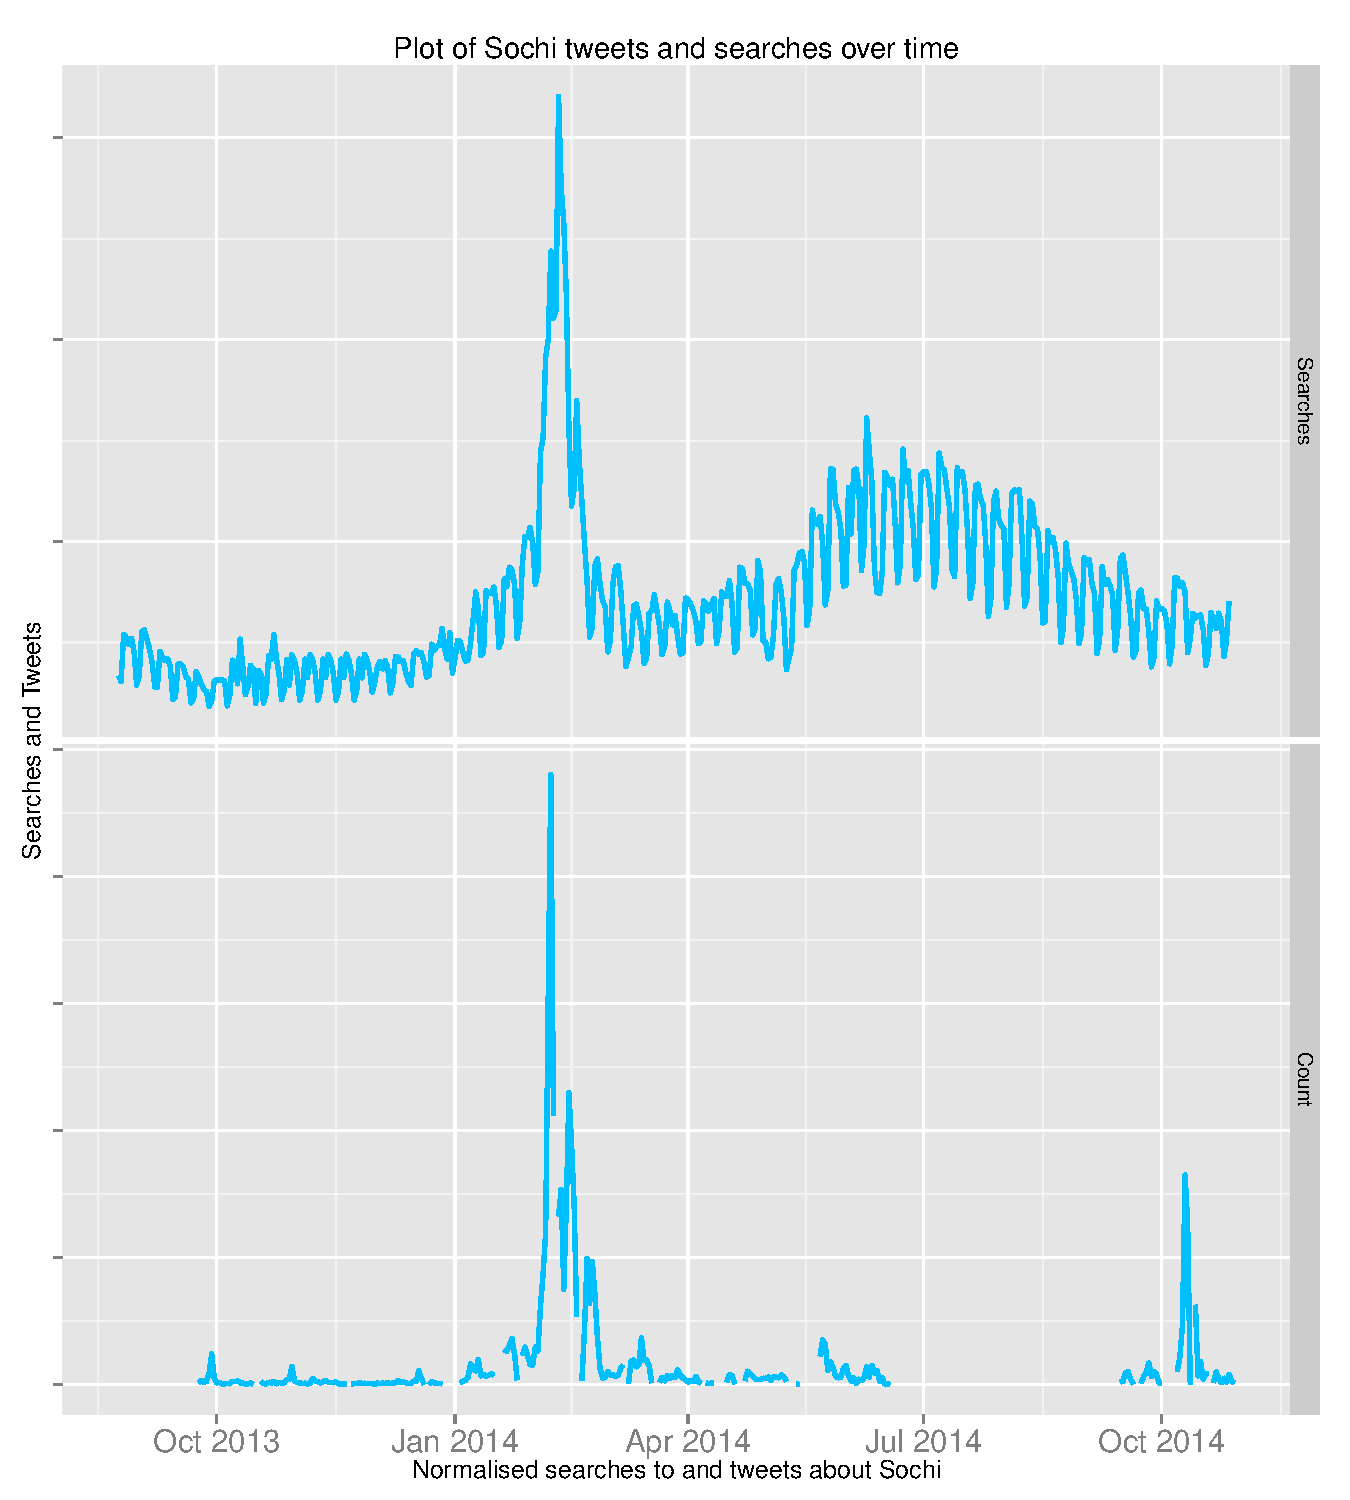
\includegraphics[width=\textwidth]{Sochi}
\end{center}
\caption{Searches and Counts to Sochi. Big spike corresponds to the winter olympics. }
\label{sochifinalplot}
\end{figure}

\begin{figure}[p!]
\begin{center}
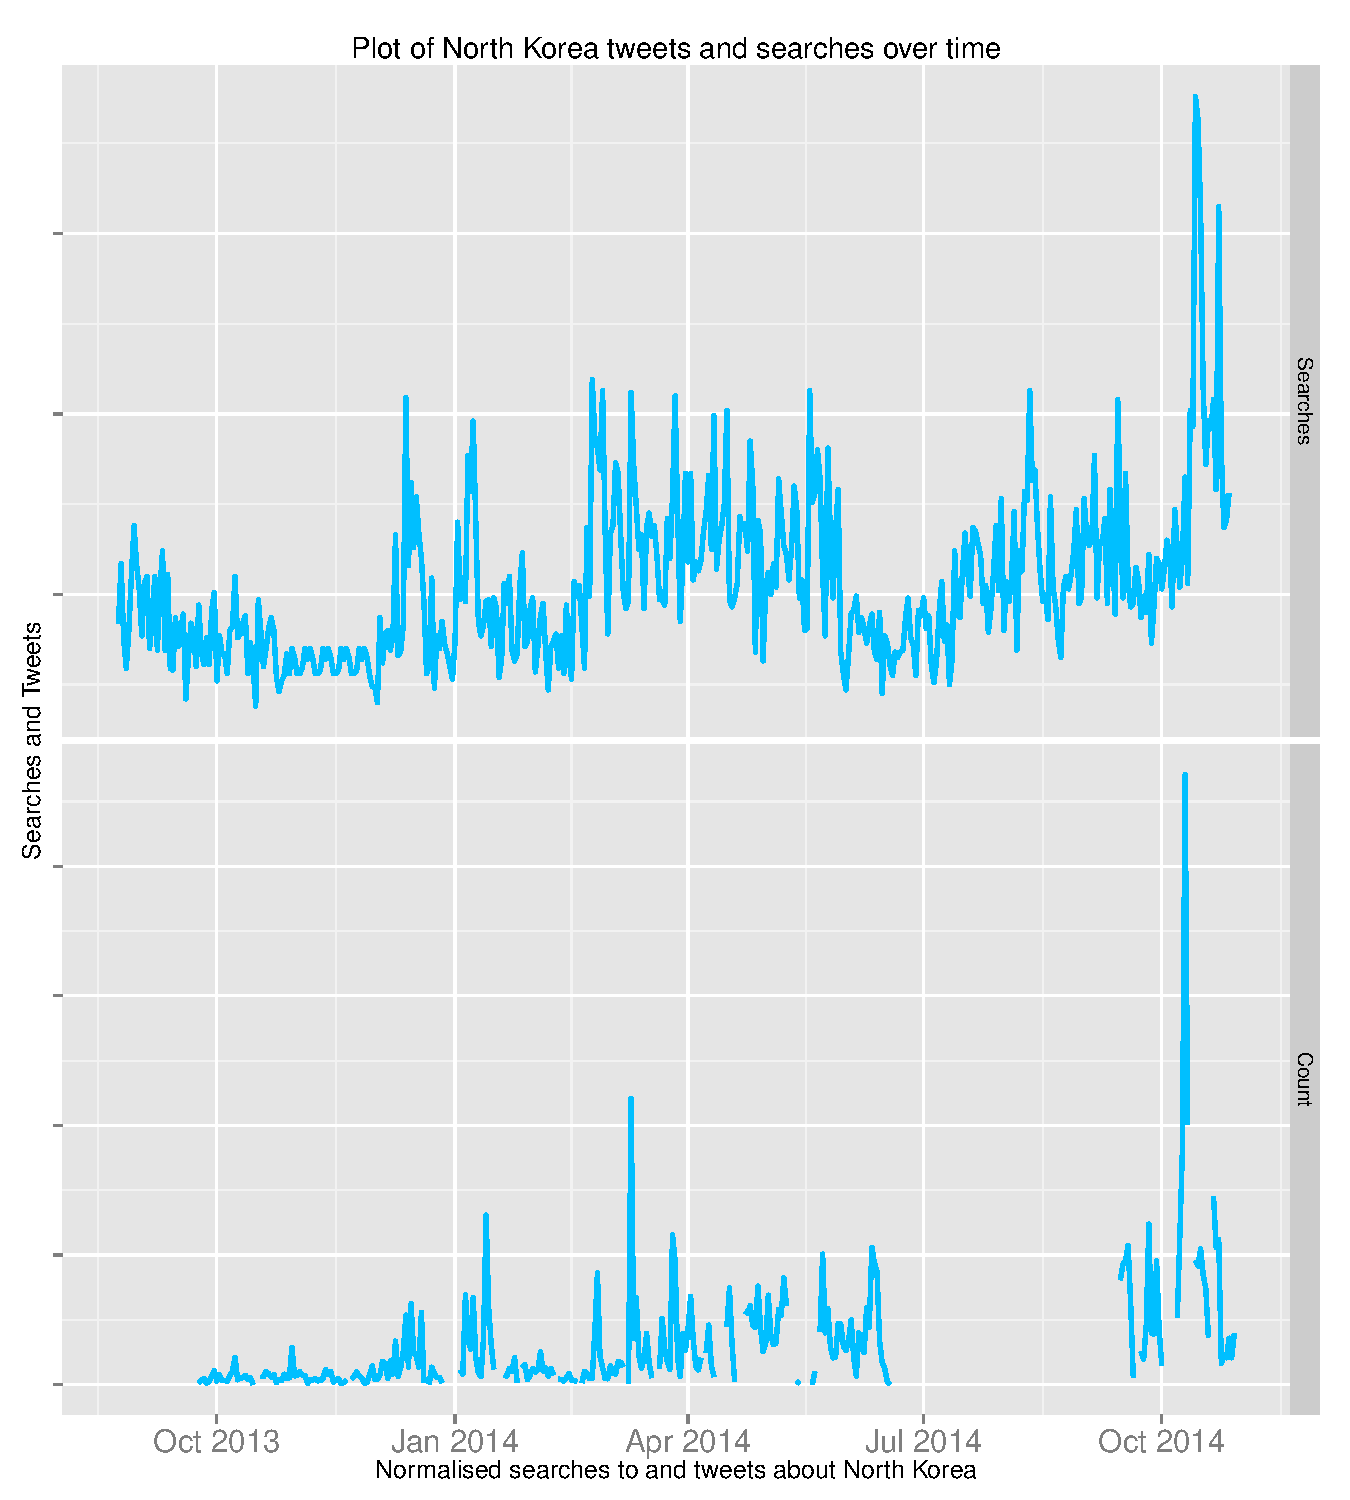
\includegraphics[width=\textwidth]{North_Korea}
\end{center}
\caption{Searches and Counts to North Korea. Notice the step change. }
\label{NorthKoreaPlot}
\end{figure}

The way those are creates is simple:
\begin{itemize}
\item We take all weekly coefficients setting Monday to be 1 and every day of the week a multiplier of that. 
\item We sample a random number from a normal distribution. We then get the whole week by multiplying this number by the coefficients and add some noise to the data. 
\item Add step changes, gradual increases and various other patterns to the data to the change point methods.
\end{itemize}

\section{ARIMA vs L4F}

The first things, that we set out to benchmark was to see whether ARIMA would outperform Last 4 Fridays for the majority of the  destinations. However our approach to the testing set was rather different this time. Since Last 4 Fridays in general works well enough on the destinations without any major changes in their profiles.

However, after all, in this work, we are not concerned with the general cases, but rather with those outliers that skew the statistic, for the very fact that they are the ones that have something interesting happened in them. Results for the smaller set of destinations without the change point time series segmentation can be found in Table \ref{comparison-results-v1}. 

\begin{table}[h!]
\begin{center}
\begin{tabular}{ l | r  | r}
Place & L4F & ARIMA\\
\hline
Brazil & 8158.84 & 4539.08\\
Sochi & 3410.60 & 1663.69\\
Fukuoka & 255.36 & 158.50\\
Ukraine & 6349.47 & 3165.19\\
Venezuela & 590.07 & 395.45\\
Sevastopol & 316.10 & 182.34\\
North Korea & 44.83 & 34.99\\
Uruguay & 349.67 & 278.89\\
\hline
\textbf{Median} & \textbf{469.87} & \textbf{337.17} \\
\hline
\textbf{Mean} & \textbf{2434.37} & \textbf{1302.27}\\
\end{tabular}
\end{center}
\caption{Results on the small set of places without change point detection. The numbers are RMSE errors.}
\label{comparison-results-v1}
\end{table}

The methodology for this test was the following:
\begin{enumerate}
\item We take 330 data points (nearly a year) from the 400 we have available. 
\item We fit the ARIMA on those data points. 
\item We forecast the next 70 days with both the L4F and ARIMA.
\item We record the Root Mean Squared Error (RMSE) for both. 
\end{enumerate}
Taking all of this we ran the test and the results were the following - the simple ARIMA yields an improvement of 46\% on the mean and 28\% on the median RMSE. That is a rather good result and we are confident that the change point segmentation of the time series would improve things even further. 

The next step in our working was to check whether the results are statistically significant or they have occurred by change. In order to see whether the results are indeed significant we used the Wilcoxon signed test and the Student t-test. Both results are pretty standard as far as statistical significance of results is concerned. The Wilcoxon signed test is a version of the signed test that tests 2 paired results to see whether the improvements is purely by coincidence. The t-test is another classic statistical test that checks significance. The p-value from the the Wilcoxon signed test is \textbf{0.007} and the paired t-test returned a p-value of \textbf{0.03}. Both values are statistically significant, so that meant that we could continue pursuing this avenue of work for the rest of the project. 

\section{Change point detection}

The next things that we had to check was the change point detection algorithm. For the destinations that we used to test it on it performed rather well. As we mentioned in Section 5.1, we had generated some data to test whether the algorithm was working as it should.

In order to do that test we had to manually go through those 20 generated datasets and label the change points we'd like. For us those were:
\begin{itemize}
\item A step change;
\item A gradual or sudden increase/decrease.
\end{itemize}
That was rather laborious, but we manage to map all of those and to run the algorithm on all. For the purposes of the tests we used only the online version, since it was much faster and much better fit for the job. 

After accumulating all the False Positives, True Positives statistic we had the data for the 20 data points. The FP vs Recall plot can be found in Figure \ref{fprecall}. As we can see overall the performance of the algorithm does not decrease greatly, but with more false positives recall is getting worse as well. In Figure 4.10 we had another example of the change point detection over north Korea. It managed to correctly frame the first peak, the step change in the time series around the middle and then it managed to predict correctly the biggest peak and flag it up as a change point however it seems that as you're acquiring more and more data perhaps the test needs to be tweaked ever so slightly to account for the fact that you've got more data.


\begin{figure}[h!]
\begin{center}
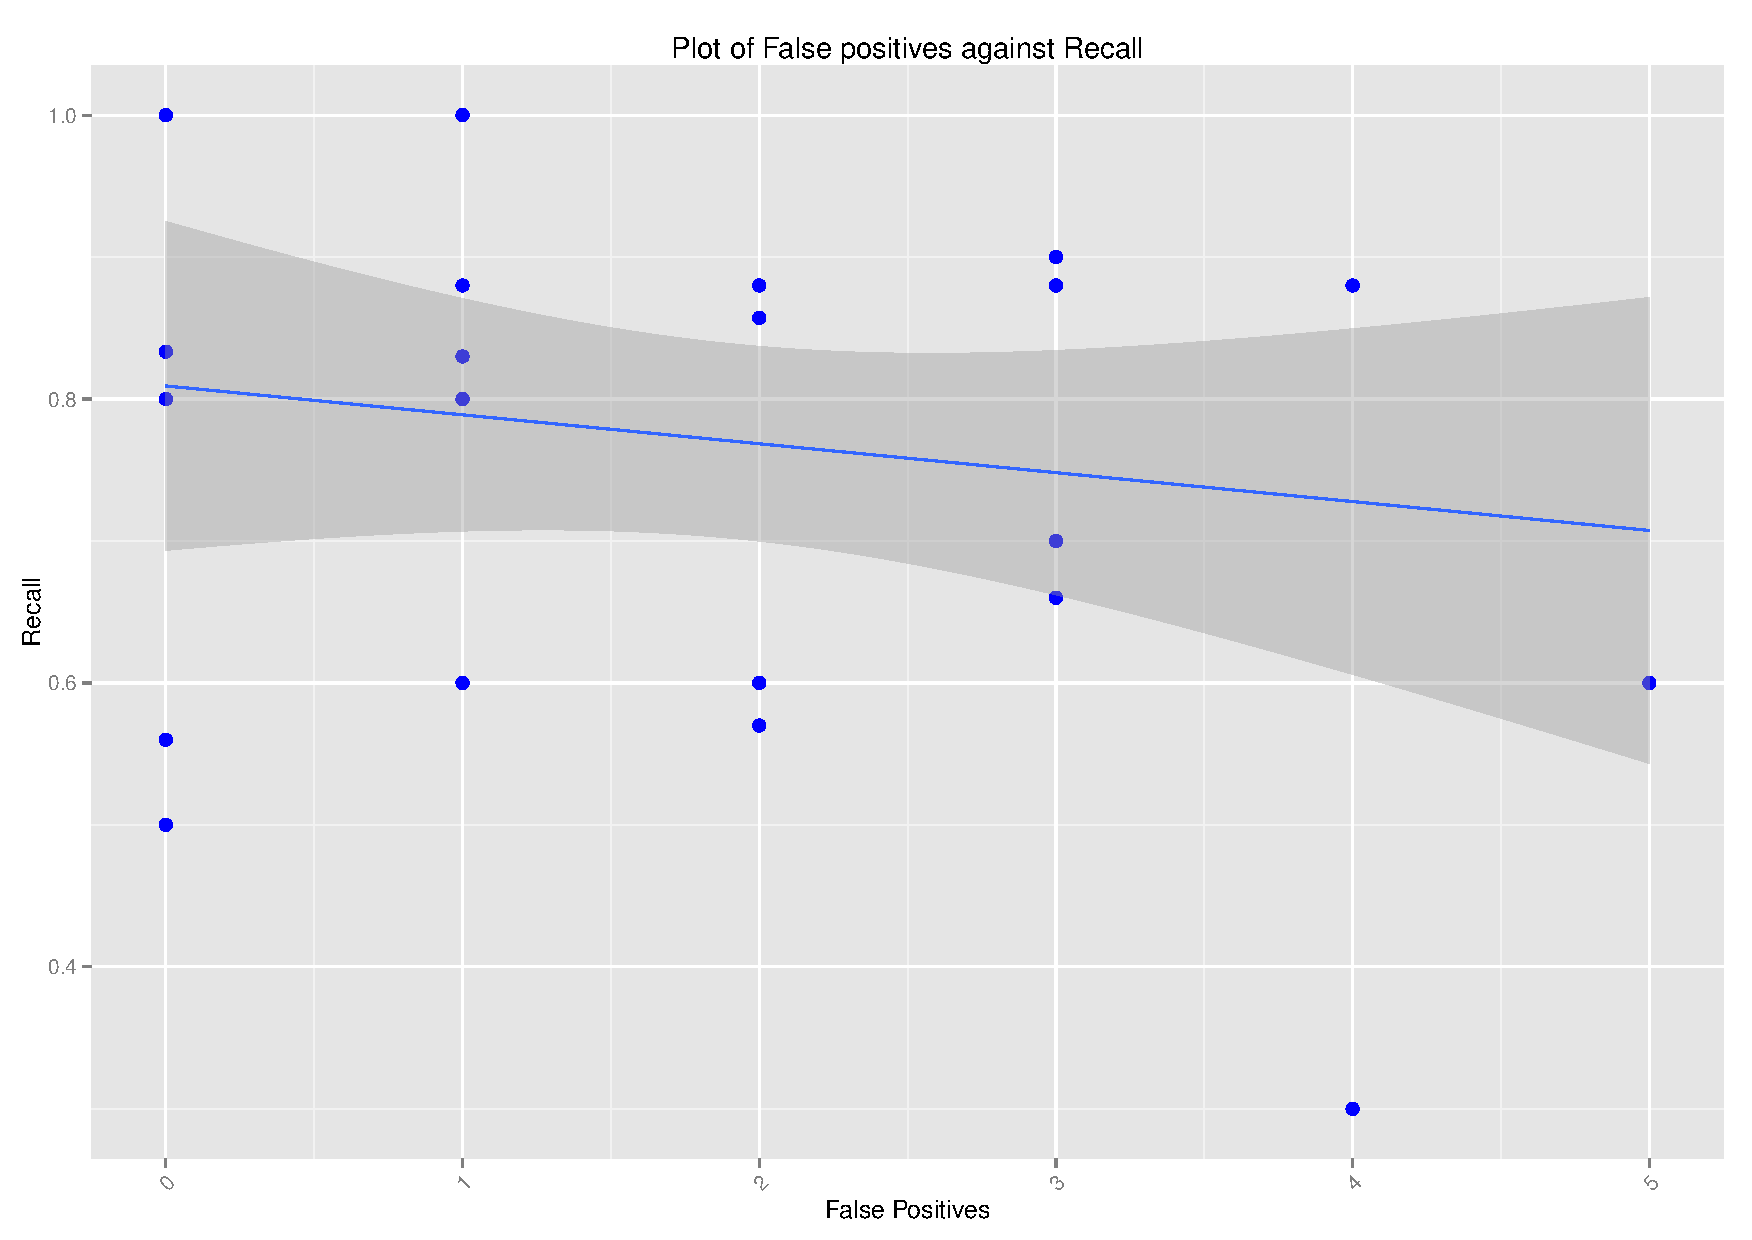
\includegraphics[width=\textwidth]{FP_vs_Recall}
\end{center}
\caption{Recall vs FP plot. As you can see the performance of the algorithm does not decrease much for more false positives.}
\label{fprecall}
\end{figure}

The results from this were promising, since it seemed that the algorithm could definitely be used to improve the forecasts produced by ARIMA by segmenting the data and fitting an ARIMA to each segment separately.

\section{Improvement with change points}

Since the change point algorithm worked rather well the next step was to see whether it would help with making the forecasts. The methodology was quite similar to the one that is described in Section 5.2 with one exception - every time there is a change point we would fit an ARIMA to each segment. Then for the 20\% data that we get the test statistic from we run the change point algorithm and if a change point happens we fit a different model again and continue with the forecasting.

The results for this can found in Table \ref{comparison-results-v2}. We have shown the L4F RMSE, the ARIMA and the ARIMA models with the change points factored in. 

\begin{table}[h]
\begin{center}
\begin{tabular}{ l | r | r | r } 
Place & L4F & ARIMA & ARIMA with change points\\
\hline
Brazil	&	8158.84	&	4539.08	&	4312.13 \\
Sochi	&	3410.6	&	1663.69	&	1497.32 \\
Fukuoka	&	255.36	&	158.5	&	128.75 \\
Ukraine	&	6349.47	&	3165.19	&	2917.90 \\
Venezuela	&	590.07	&	395.45	&	360.80 \\
Sevastopol	&	316.1	&	182.34	&	162.50 \\
North Korea	&	44.83	&	34.99	&	31.49 \\
Uruguay	&	349.67	&	278.89	&	256.26 \\
\hline
\textbf{Median} & \textbf{469.87} & \textbf{337.17}  & \textbf{308.55}\\
\hline
\textbf{Mean} & \textbf{2434.37} & \textbf{1302.27} & \textbf{1208.34}\\
\end{tabular}
\end{center}
\caption{Extended results set including the ARIMA with change points.}
\label{comparison-results-v2}
\end{table}

\section{Results overview}
An overview of the results:
\begin{itemize}
\item The improvement of median RMSE between L4F and the ARIMA models with change points is 34.33\%, while the improvement on the average RMSE is 49.64\%. 
\item The improvement form the ARIMA with and the ARIMA without change points is 8.5\% on the median RMSE across the destinations and 7.5\% across the average RMSE. 
\item On the generated data set ARIMA with change points decreased the median RMSE by 32.3\% while the average was decreases by 45.6\% in comparison to L4F.
\end{itemize}


\chapter{Conclusion and future work}

\section{Applications at Skyscanner}

This project was done with the help of Skyscanner which provided us with the flight searches data, therefore we also need to examine what impact it will have on the company. As it currently stands they can use it for two things:
\begin{enumerate}
\item Predicting flight search volumes using either LASSO or the ARIMA models;
\item Running the algorithm to find change points in the data and by using LASSO find out what has happened.
\end{enumerate}

The ARIMA system a tits current state is not as automated as the LASSO one,so there will be a small amount of manual work, but in a week or two the system can be brought to production standards without any major efforts. As we have shown the quality of the ARIMA forecasts is much better with reduction in RMSE of up to 50\%, which is a big improvement.

When trying to quantify the impact that such an improvement would have on Skyscanner as a whole we consulted with several experts throughout the business - ranging form Business Intelligence, Finance and Marketing. Forecasts as a whole were very important for them. A 30\% improvement in the forecast accuracy could have a major impact on the way budgets are allocated - if something is happening real time and the algorithm detects it, it could be paired with a customer management system that would show targeted ads to people interesting in the event happening and thus increasing the number of people who book flights.

Having an accurate system of prediction can be quite important for the health of the service as a whole. In Chapter 1, we have outlined several high-profile outages that were caused by not knowing in terms of what's happening on the website. The work presented in here is online and by using the ARIMA with an hourly aggregation on the searches level could be used to detect whether an event or something else that has a strong effect on the flight searches is happening real-time. In order to make that even better, we could plug into other data sources such as news-wires and RSS and do article matching or simply try to extrapolate what is happening based on the most frequent words that improve the flight searches prediction.

The second way that this could be applied is not for forecast, but rather social stream monitoring. The LASSO model can be used to prune the unneeded features, the ones that do not correlate with flights searches and this way have a continuous way of monitoring what are the current words on Twitter that are correlated to flight searches and from that extrapolate what events could be happening.

\section{Conclusion}

In this project we have explored multiple approaches to adding an external factor such as Twitter into forecasting flight search volumes. This is the first work that we are aware of that has done so. We have done the following:

\begin{itemize}
\item Investigated how LASSO can be used to aid the flight searches prediction with Last 4 Fridays.
\item Developed a very automated system that can be used to collect and process Twitter Data.
\item Developed the scripts that can do the automated model building and benchmarking. 
\item Compared and tested several change point methods methods.
\item Created a new way to predict change points based on ARIMA and improved the forecasting for places with change by points by 45.6\%.
\end{itemize}

One of the things that need to be taken into account is the fact that while the first phase of the project presented a work that is generic and could be used across every single place the 2nd part has done the complete opposite - we've focused on a few destinations, created an algorithm that can detect change points and improve the forecast for those places that do have them.

The ARIMA models in itself yielded a much better improvement over Last 4 Fridays in comparison to the LASSO models we had in the first phase of the project. Therefore the first thing that should be done is to fit ARIMAs for the overall level of searches and see how accurate that is. Since it is performing well without the change point detection of places that do have them, we would expect ARIMA to yield a similar decrease as the one posted in the results in Figure \ref{comparison-results-v1} and \ref{comparison-results-v2}. 


Perhaps another avenue of work that could be explored even further is to find new and interesting ways to incorporate Twitter into the whole process and automate the prediction even further. In the first phase of the project we used the LASSO model to trim all the unnecessary features and then to give the weights. Perhaps the features could be then used as an input for a Vector AutoRegressive (VAR)\footnote{http://en.wikipedia.org/wiki/Vector\_autoregression} model that could be used for the forecasts. 

Another area which could increase the performance of the regression models and therefore improve the forecasts is feature engineering. In this particular work we have taken a rather simple approach to the problem, without putting too much effort into processing the data in other ways. What we've done is simply take all the place names that co-occur with different travel words and we've taken those raw counts and used them for the forecasts. Perhaps by exploring more in that area one would be a blue to achieve increased performance without changing much the models in the back-end, but rather improve by simply improving the inputs.

In Section 4.3 we've also presented some of the findings when we used the \textbf{bcp} package in R. An area where we think there will be a certain improvement is implementing our own Bayesian Change Point detection algorithm. By using a better prior we will be able to make the algorithm much more flexible and therefore much more well tailored for the problem we have. 

\raggedright
\sloppy
\bibliographystyle{unsrt}
\bibliography{master}

\end{document}